\documentclass[10pt]{article}
%\documentclass[10pt]{book}

\usepackage[draft]{fixme}

\usepackage{listings}
\usepackage{html}
\usepackage{color}
\usepackage{multicol}
\usepackage{multirow}
\usepackage{graphicx}
\usepackage{alltt}
% style for code listing
\lstset{language={C},basicstyle=\scriptsize} 
\newcommand{\hlstd}[1]{\textcolor[rgb]{0,0,0}{#1}}
\newcommand{\hlkey}[1]{\textcolor[rgb]{0,0,0}{\bf{#1}}}
\newcommand{\hlnum}[1]{\textcolor[rgb]{0.16,0.16,1}{#1}}
\newcommand{\hltyp}[1]{\textcolor[rgb]{0.51,0,0}{#1}}
\newcommand{\hlesc}[1]{\textcolor[rgb]{1,0,1}{#1}}
\newcommand{\hlstr}[1]{\textcolor[rgb]{1,0,0}{#1}}
\newcommand{\hldstr}[1]{\textcolor[rgb]{0.51,0.51,0}{#1}}
\newcommand{\hlcom}[1]{\textcolor[rgb]{0.51,0.51,0.51}{\it{#1}}}
\newcommand{\hldir}[1]{\textcolor[rgb]{0,0.51,0}{#1}}
\newcommand{\hlsym}[1]{\textcolor[rgb]{0,0,0}{#1}}
\newcommand{\hlline}[1]{\textcolor[rgb]{0.33,0.33,0.33}{#1}}

\newcommand{\mySmallFontSize}{\scriptsize}
\newcommand{\mySmallestFontSize}{\tiny}

\newcommand{\codeFontSize}{\scriptsize}
\newcommand{\code}[1]{{\scriptsize #1}}

% Software version number
%\newcommand{\VersionNumber}{@VERSION@}

%\newcommand{\ExampleDirectory}{@top_srcdir@/projects/compass/tests}

% Latex trick to allow us to comment out large sections of documentation
\newcommand{\commentout}[1]{}

% change the title of the Fixme List
\renewcommand{\listfixmename}{Things to Fix in Documentation}

\newcommand{\comm}[2]{\bigskip
                      \begin{tabular}{|p{11cm}|}\hline
                      \multicolumn{1}{|c|}{{\bf Comment by #1}}\\ \hline
                      #2\\ \hline
                      \end{tabular}
                      \bigskip
                     }

\def\verbatimfile#1{\begingroup
                    \@verbatim \frenchspacing \@vobeyspaces
                    \input#1 \endgroup
}

\newcounter{lineno}

% Taken from verbatimfiles.sty on web
\makeatletter %JCL

\def\verbatimlisting#1{\setcounter{lineno}{0}%
    \begingroup \@verbatim \frenchspacing \@vobeyspaces \parindent=20pt
    \everypar{\stepcounter{lineno}\llap{\thelineno\ \ }}\input#1
    \endgroup
}

\makeatother %JCL

% \endinput

\addtolength{\textheight}{0.5in}
\sloppy

%---------------------------------------------------------------------
% Begin Document
%---------------------------------------------------------------------

\begin{document}

% This draft mode eliminates the figures (leaves boxes for where they would be)
%\textcolor{green}{(Associated with ROSE Version @VERSION@)} } }
%\psdraft

\title{ {\bf \textcolor{red}{A ROSE-Based End-to-End Empirical Tuning
  System for Whole Applications} \\ 
              \textcolor{blue}{Draft User Tutorial} \\
%              \textcolor{green}{(Associated with ROSE Version @VERSION@)} 
              } }
\author{ {\bf Chunhua Liao and Dan Quinlan} \\
         Lawrence Livermore National Laboratory \\ 
         Livermore, CA  94550 \\
         925-423-2668 (office)  925-422-6278 (fax) \\
         \{liao6, quinlan1\}@llnl.gov \\
         Project Web Page:
         \htmladdnormallink{http://www.rosecompiler.org}{http://www.rosecompiler.org} \\
         UCRL Number for ROSE User Manual: UCRL-SM-210137-DRAFT \\
         UCRL Number for ROSE Tutorial: UCRL-SM-210032-DRAFT \\
         UCRL Number for ROSE Source Code: UCRL-CODE-155962 \\ \\
         \htmladdnormallink{ROSE User Manual
         (pdf)}{http://www.rosecompiler.org/ROSE_UserManual/ROSE-UserManual.pdf} \\
         \htmladdnormallink{ROSE Tutorial
         (pdf)}{http://www.rosecompiler.org/ROSE_Tutorial/ROSE-Tutorial.pdf} \\
         \htmladdnormallink{ROSE HTML Reference (html
         only)}{http://www.rosecompiler.org/ROSE_HTML_Reference/index.html}
       }
\maketitle
\newpage


% This fixes the really long table of contents problem
\setcounter{tocdepth}{2}

\tableofcontents
\newpage
%

%\chapter{Introduction}
\section{Introduction}
This document describes an on-going project aimed for a
ROSE~\cite{roseWeb2008}-based end-to-end empirical tuning (also called
    autotuning) system. 
It is part of an SciDAC PERI~\cite{peri} project to enable performance
portability of DOE applications through an empirical tuning system.
Our goal is to incorporate a set of external tools interacting with
ROSE-based components to support the entire life-cycle of automated empirical optimization.
We strive to keep this document up-to-date for better communication among
project participants. 
This document is not meant to reflect the final design or implementation choices. 

% moved to later sections, Liao, 8/4/2009
%\begin{figure}[htbp]  
%	\centering
%		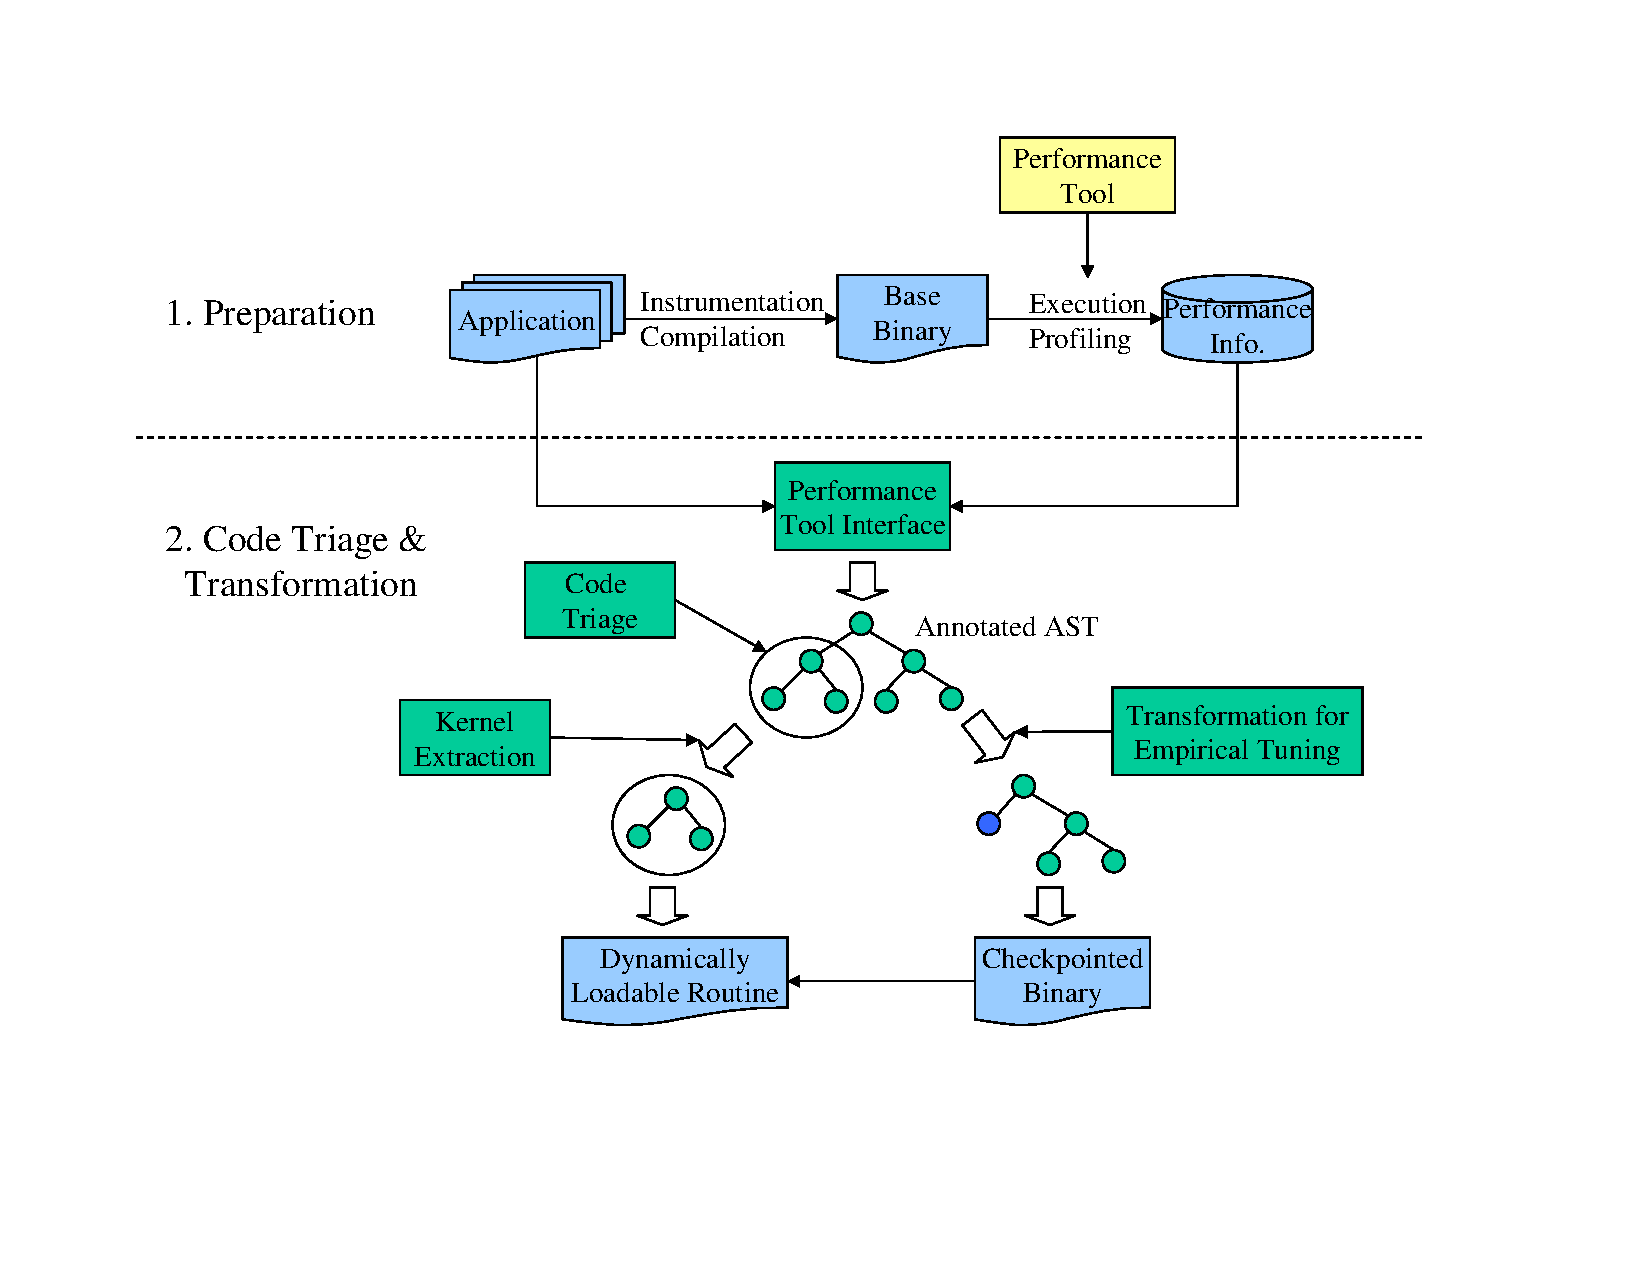
\includegraphics[width=1.2\textwidth]{phase12.pdf}
%	\caption{Phase 1 and 2 of the autotuning system}
%	\label{fig:phase12}
%\end{figure}
%
%\begin{figure}[htbp]  
%	\centering
%		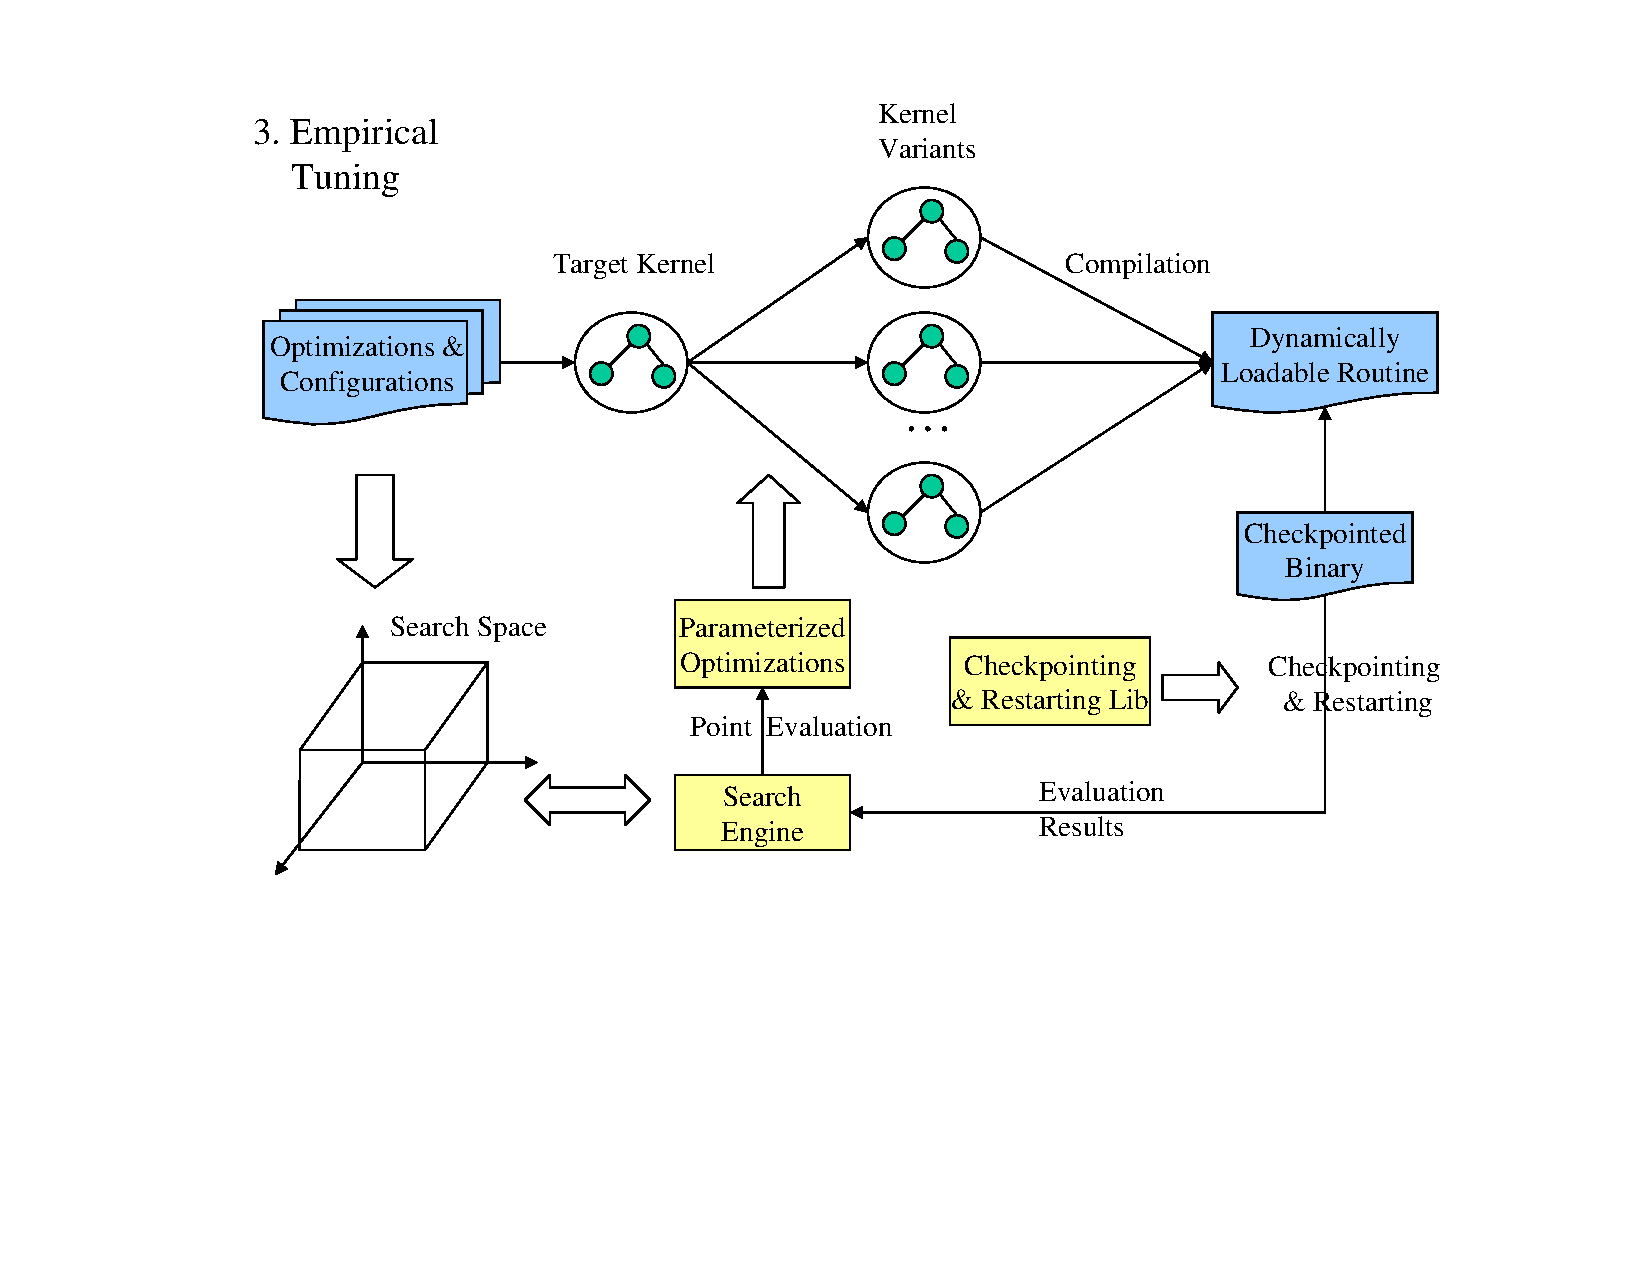
\includegraphics[width=1.2\textwidth]{phase3.pdf}
%	\caption{Phase 3 of the autotuning system}
%	\label{fig:phase3}
%\end{figure}

Currently, the ROSE-based autotuning system (shown in
    Fig.~\ref{fig:autotuning-overview}) is designed to work in three major
phases. 
%(Phase 1 and 2 are shown in Fig.~\ref{fig:phase12} and phase 3 is shown 
%in Fig.~\ref{fig:phase3}). 

\begin{figure}[htbp]  
                \vspace{-15ex}
	\centering
		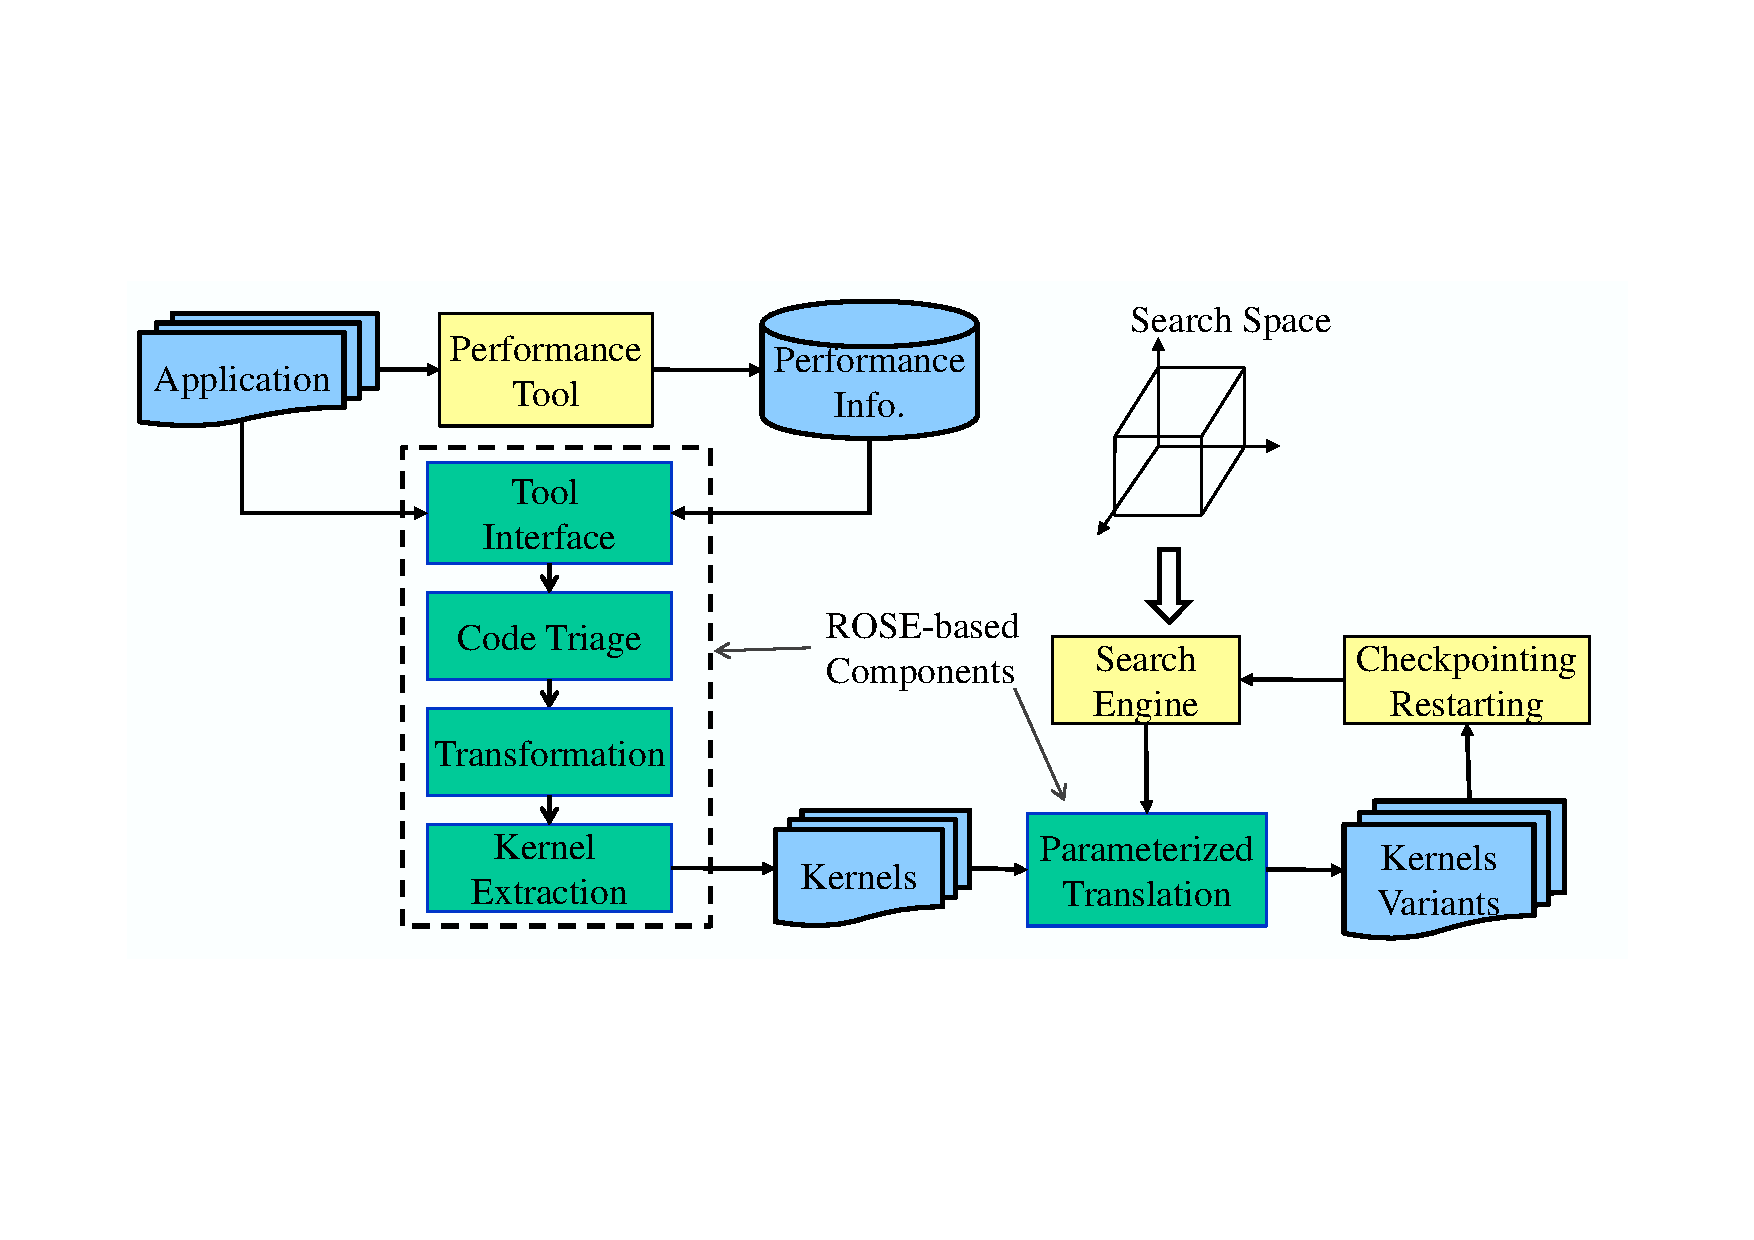
\includegraphics[width=1.2\textwidth]{rose-autotuning-overview.pdf}
                \vspace{-15ex}
	\caption{A ROSE-based end-to-end autotuning system}
	\label{fig:autotuning-overview}
\end{figure}


\begin{enumerate}
% It starts with a preparation phase by using external performance tools to collect basic performance metrics of a target application. 
   \item {\bf Preparation} \\ 
      The preparation phase uses external performance tools to collect basic performance
      metrics of a target application. 

   \item {\bf Code triage, kernel extraction and transformations} \\
      This phase is carried out by a set of ROSE-based modules. 
      A ROSE tool interface
      module reads in both source files of the application and the performance data to
      construct an abstract syntax tree (AST) representation of the input code annotated
      with performance information. 

      Then a code triage module is followed to locate problematic targets (e.g
      loops) within the application. A set of potentially beneficial
      optimizations and/or their configurations for each target is chosen
      (manually for now) based on program analysis. 
% The remaining process is repeated for each target in order to find an
%optimal optimization solution. 

      After that, a ROSE AST Outliner extracts a selected target into
      a stand-alone kernel, which will in turn be compiled into a dynamically loadable library routine. 
      The application will be transformed accordingly and compiled to be a binary executable.
      This binary executable calls the outlined routine, collects performance metrics for
      the call.
      Optionally, a checkpointing/restarting library can be used to shorten
      the execution by stopping (checkpointing) and
      restarting immediately before calling the outlined function.

   \item {\bf Empirical tuning} \\
      The final phase does the actual empirical tuning. First of all, the
      potentially beneficial optimizations and their corresponding configurations
      are represented as points within an integral search space which can be handled by a search engine. 
      The search engine adopts some search policy to evaluate points in the search space
      and search for a point corresponding a transformation strategy leading to the best
      performance. 

      During this phase, multiple versions of the target kernel are generated by
      a parameterized translator%(e.g. a ROSE-based Loop Optimizer or other parameterized optimizers)
      from the searched points and compiled into dynamically loadable library
      routines. The performance of the kernel variants are measured one by one as the
      checkpointed binary is restarted multiple times and calls multiple versions
      of the dynamically loadable library routine. 
\end{enumerate}

We give some details about the system design and the current implementation
status in the following sections. 

A list of our current hardware/software configurations is given below:
\begin{itemize}
   \item A Dell Precision T5400 workstation with two sockets, each a 3.16
   GHz quad-core Intel Xeon X5460 processor, and total 8 GB memory; 
   \item Red Hat Enterprise Linux release 5.3 (Tikanga) Linux x86 kernel
   2.6.18-92.el5.perfctr SMP PREEMPT;
   \item PAPI 3.6.2;
   \item the Rice HPCToolkit version TRUNK-4.9.0=1280 (the latest
         release does not support the 32-bit machine we use, so we use an
         older version); 
   \item ROSE compiler version 0.9.4a, revision 6701 (providing a tool
       interface, outliner, loop translator, etc.);
   \item Berkeley Lab Checkpointing and Restarting library V. 0.8.2;
   \item POET from Univ. Texas San Antonio (We use its latest CVS version
         actually, not sure the exact release version number);
   \item the GCO search engine from Univ. of Tennessee (UTK) (We got a package from
         UTK directly, not sure the release number); 
%(Only an old version provided by UTK  works with the search engine right now).
   \item a C version jacobi iteration program, used as a simple example
   input code for autotuning.      

   \item the SMG2000~\cite{BrownSemicoarsening2000} (Semicoarsening Multigrid
         Solver) benchmark from the ASCI Purple, used as an example real
         application.
\end{itemize}



\clearpage
%\newpage
\section{Preparation}
The preparation phase provides basic information about a target application's performance
characteristics. 
Such information can be obtained by many performance tools.
Currently, we accept performance data generated by both HPCToolkit and GNU gprof.
%Currently, the ROSE-HPCToolKit interface is used to accept performance data generated by HPCToolkit and GNU gprof.
%The interface is used to annotate ROSE AST with performance metrics to
%facilitate building automated performance analysis tools. 
%Detailed information about ROSE-HPCToolKit can be found in Chapter 44 of
%the ROSE tutorial. 
%We only give information relevant to autotuning below.

\subsection{Using HPCToolkit}
%The HPCToolkit~\cite{hpctoolkit} is developed at the Rice University to get
%performance metrics of the target application. 
The HPCToolkit~\cite{hpctoolkit}, developed at the Rice University, is an open source profile-based
performance analysis tool which samples the executions of optimized applications. 
No code
instrumentation is needed to use HPCToolkit. 
But debugging information (by compiling with
the -g option if GCC is used) in the binary executables is needed for the tool to
associate performance metrics with source language constructs.

After installation, a typical session of using HPCToolkit is given below:
{\mySmallFontSize
\begin{verbatim}
% Prepare the executable with debugging information
gcc -g smg2000.c -o smg2000 

% Sample one or more events for the execution, use wall clock here
hpcrun -e WALLCLK -- ./smg2000 -n 120 120 120 -d 3

% Convert the profiling result into a XML format
hpcproftt -p -D /home/liao6/svnrepos/benchmarks/smg2000 ./smg2000 \
  smg2000.WALLCLK.tux268.llnl.gov.10676.0x0 > result.xml

\end{verbatim}
}

\fixme{TODO: update the text when the latest release of HPCToolkit works
on 32-bit platforms}

%A SMG2000~\cite{BrownSemicoarsening2000} (Semicoarsening Multigrid Solver) benchmark from the ASCI Purple
%benchmark suite is chosen to exemplify the use of this system.

Fig.~\ref{fig:hpctoolkitSmg2000} shows the profiling results of SMG2000
using HPCToolkit. 
A statement in a loop takes more than 46\% execution time, which makes the
loop dominant, most expensive loop of the entire program.
\begin{figure}[htbp]  
	\centering
		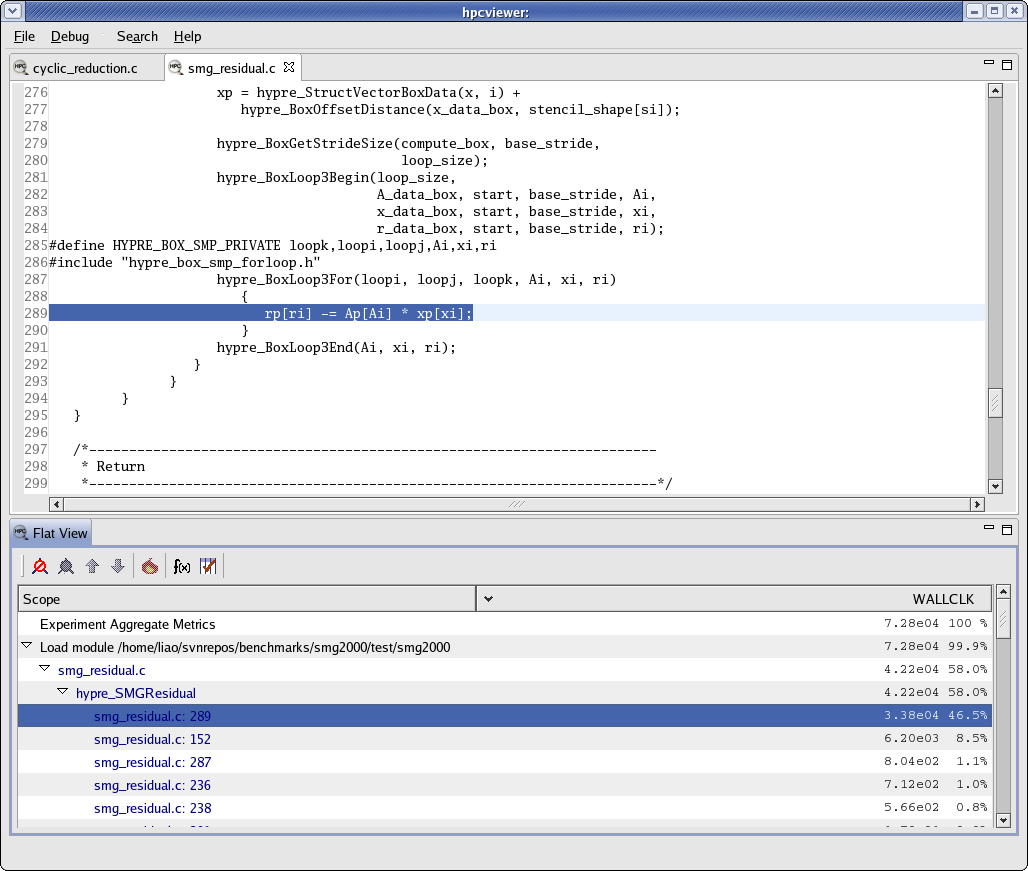
\includegraphics[width=0.9\textwidth]{hpctoolkit-smg2000.png}
	\caption{Profiling results of SMG2000 using HPCToolkit}
	\label{fig:hpctoolkitSmg2000}
\end{figure}

\subsection{Using gprof}
GNU gprof can generate line-by-line performance information for an
application. A typical session to generate such information is given below:
\begin{verbatim}
[liao@codes]$ gcc -g seq-pi.c -pg
[liao@codes]$ ./a.out
[liao@codes]$ gprof -l -L a.out gmon.out &>profile.result
\end{verbatim}

The option {\tt -l} tells gprof to output line-by-line profiling
information. 
{\tt -L} causes gprof to output full file path information, which is needed
for ROSE to accurately match performance data to source code.

An excerpt of an output file for smg2000 looks like the following:
{\scriptsize
\begin{verbatim}
Flat profile:

Each sample counts as 0.01 seconds.
  %   cumulative   self     
 time   seconds   seconds     name
 35.01     13.08    13.08     hypre_SMGResidual (/home/liao/smg2000/struct_ls/smg_residual.c:289 @ 804caa4)
  9.05     16.46     3.38     hypre_CyclicReduction (/home/liao/smg2000/struct_ls/cyclic_reduction.c:1130 @ 8054af4)
  8.40     19.60     3.14     hypre_SMGResidual (/home/liao/benchmarks/smg2000/struct_ls/smg_residual.c:291 @ 804cab9)
  7.67     22.46     2.87     hypre_CyclicReduction (/home/liao/smg2000/struct_ls/cyclic_reduction.c:910 @ 8053191)
  5.97     24.70     2.23     hypre_CyclicReduction (/home/liao/smg2000/struct_ls/cyclic_reduction.c:998 @ 8053a28)
  5.27     26.66     1.97     hypre_SMGResidual (/home/liao/smg2000/struct_ls/smg_residual.c:238 @ 804d129)
  2.86     27.73     1.07     hypre_SMGResidual (/home/liao/smg2000/struct_ls/smg_residual.c:287 @ 804cacb)
  2.28     28.59     0.85     hypre_CyclicReduction (/home/liaosmg2000/struct_ls/cyclic_reduction.c:853 @ 8052bae)
  2.07     29.36     0.78     hypre_CyclicReduction (/home/liao/smg2000/struct_ls/cyclic_reduction.c:1061 @ 8054450)
  1.79     30.03     0.67     hypre_SemiRestrict (/home/liao/smg2000/struct_ls/semi_restrict.c:262 @ 8056a8c)
  1.67     30.66     0.62     hypre_SemiInterp (/home/liao/smg2000/struct_ls/semi_interp.c:294 @ 8055d6c)
  1.12     31.07     0.42     hypre_CyclicReduction (/home/liao/smg2000/struct_ls/cyclic_reduction.c:1133 @ 8054b2f)
  0.96     31.43     0.36     hypre_CyclicReduction (/home/liao/smg2000/struct_ls/cyclic_reduction.c:912 @ 80531a6)
  0.87     31.76     0.33     hypre_StructAxpy (/home/liao/smg2000/struct_mv/struct_axpy.c:69 @ 806642c)
  0.80     32.06     0.30     hypre_CyclicReduction (/home/liao/smg2000/struct_ls/cyclic_reduction.c:1002 @ 8053a60)
  0.78     32.35     0.29     hypre_SMGResidual (/home/liao/smg2000/struct_ls/smg_residual.c:236 @ 804d14b)
  0.72     32.62     0.27     hypre_CyclicReduction (/home/liao/smg2000/struct_ls/cyclic_reduction.c:1063 @ 8054462)
  0.60     32.84     0.23     hypre_SMGAxpy (/home/liao/smg2000/struct_ls/smg_axpy.c:69 @ 8064970)
  0.59     33.06     0.22     hypre_CycRedSetupCoarseOp (/home/liao/smg2000/struct_ls/cyclic_reduction.c:369 @ 8051149)
  0.59     33.28     0.22     hypre_SMGResidual (/home/liao/smg2000/struct_ls/smg_residual.c:240 @ 804d146)
  0.51     33.48     0.19     hypre_StructVectorSetConstantValues (/home/liao/smg2000/struct_mv/struct_vector.c:578 @ 806fedc)
  0.48     33.66     0.18     hypre_SMGSetupInterpOp (/home/liao/smg2000/struct_ls/smg_setup_interp.c:292 @ 804ea04)
  0.46     33.83     0.17     hypre_SemiInterp (/home/liao/smg2000/struct_ls/semi_interp.c:227 @ 80556e8)
  0.40     33.98     0.15     hypre_CyclicReduction (/home/liao/smg2000/struct_ls/cyclic_reduction.c:855 @ 8052bd4)
  0.40     34.12     0.15     hypre_StructMatrixInitializeData (/home/liao/smg2000/struct_mv/struct_matrix.c:359 @ 80678b0)
  ...
\end{verbatim}
}



%We use the self seconds associated with each source line and attach them to
%ROSE AST as AST attributes named WALLCLK.


\clearpage
\section{Code Triage and Transformations}
The second phase (shown in Fig.~\ref{fig:phase12}) includes code triage and a set of code transformations. 
Code triage relies on a ROSE-based tool interface to read in both source files and performance information of
the input application.
It then conducts various automated or user-directed analyses to identify
problematic code segments, such as loops. 
Finally, the identified code segments are extracted (also called outlined) into separated routines so they can be individually
optimized by empirical methods. 
%Since the analysis is on the AST or other graphs built
%using ROSE and uses the performance data stored as attributes, these analyses are
%expressed using traversals in ROSE.
\begin{figure}[htbp]
\vspace{5ex}
       \centering
               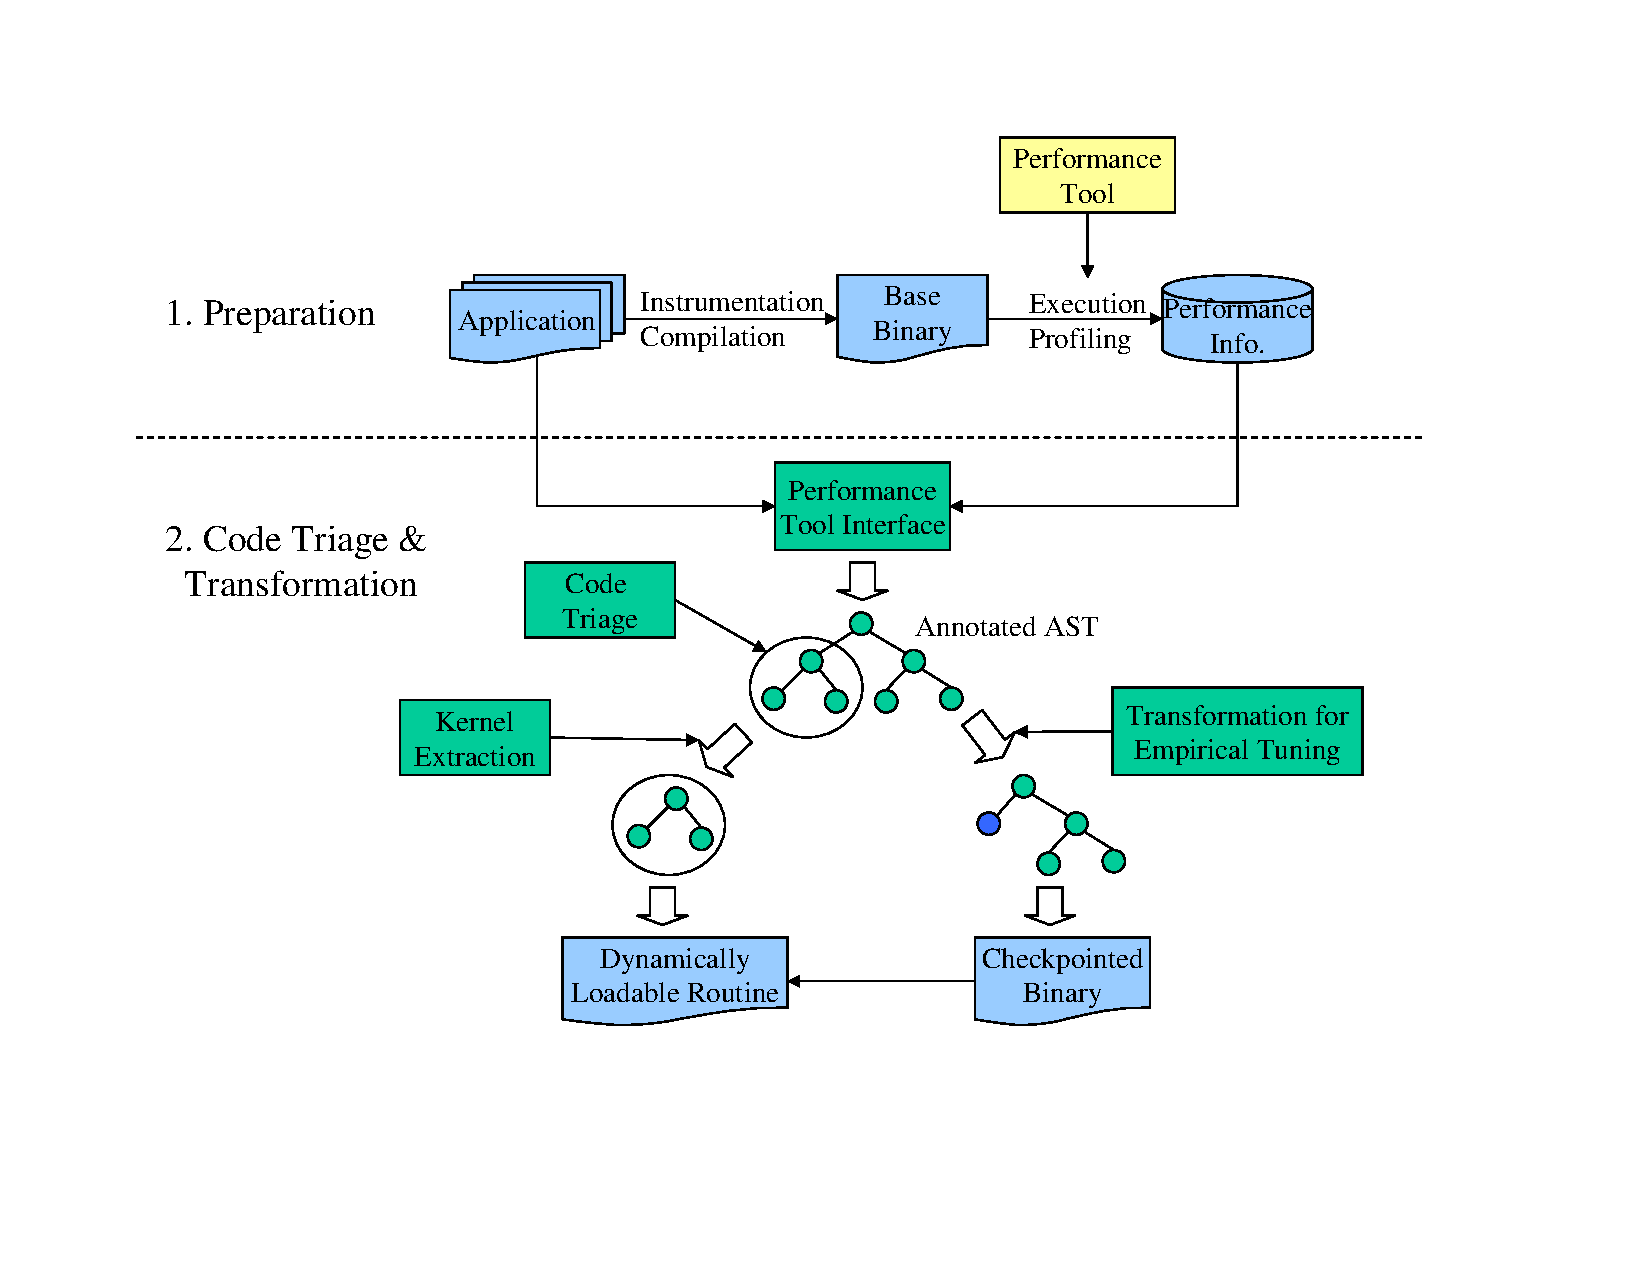
\includegraphics[width=1.2\textwidth]{phase12.pdf}
       \caption{Phase 1 and 2 of the autotuning system}
       \label{fig:phase12}
\end{figure}

%---------------------------------------------------
\subsection{Invoking Code Triage}
The source code for code triage is located in
\textit{rose/projects/autoTuning/autoTuning.C}. 
It already has initial implementation to call ROSE's tool interface,
conduct simple code triage, and finally extract kernels using ROSE's AST
outliner. 

With the input application and its performance result available, 
%a straightforward method is used to identify the most time-consuming
%statements in the code.  
%Loop nests containing those statements are reported as a
%tuning candidate, if the loop nests exist.
users can invoke the ROSE-based code triage by using the following command:

{\mySmallFontSize
\begin{verbatim}
autoTuning -c  jacobi.c -rose:hpct:prof jacobi-raw.xml \
-rose:autotuning:triage_threshold 0.8 -rose:outline:output_path "tests"
\end{verbatim}
}

The command above provides an input source file and its corresponding XML-format performance data generated by HPCToolkit.
It asks the code triage program to find the most time-consuming 
loops which account for just above 80\% of the total execution time. 
The identified loops will be automatically extracted to separated,
source files and saved into an output path named \textit{tests}.

Users can also enable code triage only without calling outlining. 
The performance data can come from GNU gprof. 
An example is given below:

%{\scriptsize
{\mySmallFontSize
\begin{verbatim}
# example command line to perform code triage only.
autoTuning  -c jacobi.c -rose:autotuning:triage_only -rose:gprof:linebyline jacobi.gprof.txt 

# the output is a list of abstract handles and 
# their corresponding execution time percentage
-----------------------------------------------------------------
The abstract handles for hot statements exceeding the threshold are:
Project<numbering,1>::SourceFile<name,/home/liao6/jacobi.c>::\
ExprStatement<position,193.9-194.76>
0.382
Project<numbering,1>::SourceFile<name,/home/liao6/jacobi.c>::\
ExprStatement<position,196.9-196.45>
0.3643
Project<numbering,1>::SourceFile<name,/home/liao6/jacobi.c>::\
ExprStatement<position,188.9-188.29>
0.11
-----------------------------------------------------------------
The abstract handles for enclosing loops for hot statements exceeding the
threshold are:
Project<numbering,1>::SourceFile<name,/home/liao6/jacobi.c>::\
ForStatement<position,190.5-198.7>
0.8189
\end{verbatim}
}

The above example command identifies a list of the most time-consuming statements and loops and reports them using abstract handles. 
The report will end once the sum of execution time of the statements or
loops reach or exceed a preset threshold (default is 75\% of the total execution time). 

We explain some details for the implementation of code triage and
autotuning-related transformations in the following subsections.
%----------------------------------------
\subsection{Tool Interface}
%A ROSE tool interface is required for understanding the performance results of each
%external performance tool. 
ROSE has a performance tool interface, called ROSE-HPCT,
in its distribution to accept performance results generated by external
performance tools .  
%Please follow the instructions from ROSE
%Tutorial's Chapter ROSE-HPCToolkit Interface to enable and use this module. 
Basically, it reads in the XML files generated from HPCToolkit and attaches performance metrics to
the ROSE AST representing the corresponding source code.
It can handle macro expansions during the metric match process.
When necessary, all performance metrics are also propagated from statement
levels to loop, function, and file levels. 
Similarly, it also accepts the line-by-line performance data generated by GNU
gprof.
%Currently, the ROSE-HPCToolKit interface is used to accept performance
%data generated by HPCToolkit and GNU gprof.
%The interface is used to annotate ROSE AST with performance metrics to
%facilitate building automated performance analysis tools. 
Detailed information about ROSE-HPCToolKit can be found in Chapter 44 of
the \htmladdnormallink{ROSE Tutorial}{http://www.rosecompiler.org/ROSE_Tutorial/ROSE-Tutorial.pdf}.
%We only give information relevant to autotuning below.

The code triage program uses the following code to invoke ROSE-HPCT.

{\mySmallFontSize
\begin{verbatim}
int main(int argc, char * argv[]) 
{
  vector<string> argvList (argv, argv+argc);
  // Read into the XML files
  RoseHPCT::ProgramTreeList_t profiles = RoseHPCT::loadHPCTProfiles (argvList);
  // Create the AST tree
  SgProject * project = frontend(argvList);
  //Attach metrics to AST , last parameter is for verbose
  RoseHPCT::attachMetrics(profiles, project,project->get_verbose()>0);
  //...
}
\end{verbatim}
}

%%----------------------------------------
%\subsection{Code Triage}
%A code triage module examines the AST annotated with
%performance metrics to locate problematic code portions (we call these code portions
%as autotuning targets).
%Currently, a straightforward top-down method is used to identify a hot spot
%in the code from the most time consuming file and then the loop nests containing such spot is reported as a
%tuning candidate, if the loop nests exist. The example code is shown below:
%\fixme{ROSE's AST merge could be used in the future to have a global view
%of AST merged from multiple source files.}
%
%{\mySmallFontSize
%\begin{verbatim}
% std::string hot_file = findHottestFile(fileMetrics);
% SgNode* hot_node=findHottestStatement(file, nodesWithMetrics);
% SgForStatement* target_loop= findTargetLoop(hot_node);
%
%\end{verbatim}
%}
%
%Code triage is also designed to suggest a set of potentially beneficial optimizations and
%their configuration ranges to improve the performance.
%\fixme{TODO need to implement this by compiler analysis. We manually 
% use the limited optimization choices, such as loop unrolling, by default for now.}
%
% DQ: Liao, what is the best entry point for me to write such a module/traversal.
% I think it would be good to have this in place before we release this document.
% I will be happy to write this part.

%----------------------------------------
\subsection{Kernel Extraction: Outlining}
Each of the identified tuning targets, often loops, will be extracted from the original code to
form separated functions (or routines). 
The ROSE AST outliner is invoked to generate such functions. 
%It replaces a block of consecutive statements with a function call to a newly generated
%function containing those statements. 
This kernel extraction step can be automatically invoked by the code triage
program or manually initiated by users via the outliner's command line
interface. 

The ROSE AST outliner handles multiple input languages, including C, C++ and
recently Fortran.  It also provides both command line and programming interfaces for users
to specify the targets to be outlined.  
Detailed information of using the ROSE outliner can be found in
Chapter 27 of the \htmladdnormallink{ROSE
Tutorial}{http://www.rosecompiler.org/ROSE_Tutorial/ROSE-Tutorial.pdf}.
You can also refer to a paper~\cite{LiaoEffective2009} for the algorithm we use to outline kernels. 
%More details of the ROSE AST outliner are
%available in the ROSE Tutorial's Chapter, Function Outlining using the AST Outliner.
For the code triage program, the programming interface of the Outliner is
used as below:

{\mySmallFontSize
\begin{verbatim}
  // recognize options for outliner
  Outliner::commandLineProcessing(argvList);
  ...
 SgForStatement* target_loop= findTargetLoop(hot_node);
 if (isOutlineable (target_loop))  
   outline(target_loop);
\end{verbatim}
}

The ROSE AST outliner accepts user options to further guide its internal
behavior. \lstinline{-rose:outline:parameter_wrapper } will wrap all
parameters of the outlined function into an array of pointers. 
\lstinline{-rose:outline:new_file} will separate the outlined function into
a new source file to facilitate external tools for further handling.
\lstinline{-rose:outline:use_dlopen} will transform the code to use
\lstinline{dlopen()} and \lstinline{dlsym()} to dynamically load the
outlined function from a library.

For the SMG2000 example, the most time-consuming loop is outlined and a call to it is used
to replace the loop in the original code. 
The loop is actually expanded from a macro
\lstinline{hypre_BoxLoop3For()}. 
ROSE is able to identify it after a bottom
up metrics propagation phase in ROSE-HPCT. 
%\fixme{Need to come up a way to automatically handle this, Should we
%do it within the outliner itself or before calling the outliner?})
The kernel extraction's result is shown in the following code listing:
\lstset{language={C},basicstyle=\scriptsize} 
\lstinputlisting{smg2000_outlined.fold.c}
\lstset{language={C},basicstyle=\small} 

%\fixme{TODO 
%   Also we should evaluate the overhead of this
%   step if the final result is an optimized function represented as a separate 
%   file (potentially disables some optimizations).  In the final assembly 
%   we could remove the dynamic linking, but the Makefile would have to be modified which
%   gets messy for an automated system.}

The ROSE outliner uses a variable cloning method to
avoid using pointer dereferencing within the outlined computation kernels. 
The method is based on usage of a variable that is passed by reference and
accessed
via pointer-dereferencing by classic outlining algorithms.
Such a variable is used either by value or by address within an outlining
target.
For the C language, using the variable by address occurs when the
address operator
is used with the variable (e.g. \lstinline{&X}).
C++ introduces one more way of using the variable by address:
associating the variable with a reference type
(\lstinline{TYPE & Y = X;} or using the variable as an argument for a
 function's parameter of a reference type).
If the variable is not used by its address,
a temporary clone variable of the same type (using \lstinline{TYPE clone;})
can be introduced to substitute its uses within the outlined function.
The value of a clone has to be
initialized properly (using \lstinline{clone = * parameter;})
before the clone participates in computation.
After the computation, the original variable must be set to the clone's
final value
(using \lstinline{*parameter = clone}).
By doing this, many pointer dereferences introduced by the classic
algorithm can be avoided.
\fixme{We are working on using liveness analysis to further eliminate unnecessary
value assignments.}

For easier interaction with other tools, the outlined function is separated
into a new source file, usually named after 
the function name.  
The ROSE outliner will recursively find and copy all dependent type declarations
into the new file to make it compilable.
For the SMG2000 example, a file named out\_1\_6755\_\_.orig.c 
is generated and it only contains the function body of \lstinline{OUT_1_6755__()}. 
This file will be transformed by a parameterized optimizer to a kernel
variant named OUT\_\_1\_\_6755\_\_.c and further compiled into a dynamically
loadable routine.

A sample makefile to generate the .so file is given below: 

{\mySmallFontSize
\begin{verbatim}
[liao@localhost smg2000] cat makefile-lib
lib:OUT__1__6755__.so
OUT__1__6755__.o:OUT__1__6755__.c
        gcc -c -fpic OUT__1__6755__.c
OUT__1__6755__.so:OUT__1__6755__.o
        gcc -shared -lc -o OUT__1__6755__.so OUT__1__6755__.o
clean:
        rm -rf OUT__1__6755__.so OUT__1__6755__.o
\end{verbatim}
}

%----------------------------------------
\subsection{Transformations for Autotuning}
The call site of the outlined function in the source code has to be further transformed to support empirical optimization. 
These transformations include:
\begin{itemize}
\item using \lstinline{dlopen()} to open a specified .so file containing
the outlined target and calling the function found in the file,
\item adding performance measuring code to time the call of the outlined target function.
\item transforming code to support checkpointing the execution right before
\lstinline{dlopen()} opening the library source file so multiple variants of the file can be used to test optimization choices empirically when the program is restarted multiple times.
\end{itemize}
%\fixme{TODO the code translations in this sub section are manually done
%now. We will start to
%implement them once the translation methods are agreed on by partners.}
%----------------------------------------
\subsubsection{Calling a Function Found in a .so File}
As mentioned earlier, the outlined function containing the target kernel is
stored in a separated source file, which will be transformed into a kernel variant
and then compiled to a dynamically loadable library. 
The original source code has to be transformed to open the library file,
find the outlined function, and finally call it using the right
parameters. An example of the resulting transformation on the function containing the
outlined loop is given below:
\lstset{language={C}, basicstyle=\scriptsize}
\lstinputlisting{smg2000_dlopen.c}

\subsubsection{Timing the Call}
The call to the outlining target kernel should be timed to get the
evaluation results during the empirical optimization. 
We instrument the call as follows to get the performance evaluation of a
kernel variant. 
More accurate and less intrusive methods based on hardware
counters can also be used in the future. 

{\mySmallFontSize
\begin{verbatim}
//save timing information into a temporary file

remove("/tmp/peri.result");
time1=time_stamp();
// parameter wrapping statements are omitted here
(*OUT__1__6755__)(__out_argv1__1527__);

time2=time_stamp();
FILE* pfile;
pfile=fopen("/tmp/peri.result","a+");
if (pfile != NULL)
{
  fprintf(pfile,"%f\n",time2-time1);
  fclose(pfile);
}
else
  printf("Fatal error: Cannot open /tmp/peri.result!\n");

\end{verbatim}
}

%----------------------------------------
\subsubsection{Checkpointing and Restarting}
In order to efficiently evaluate hundreds or even thousands of kernel
variants, we use a checkpointing and restarting method to measure the time
spent on calling the kernel without unnecessarily repeating the execution
before and after calling the kernel.  This allows the full context (state) 
of the application to be used in the evaluation of the kernel performance.
\fixme{need to discuss the drawbacks, e.g. missing cache warmup; and how that
might be addressed in the future by pushing back the checkpoint start and 
transformations to the checkpointed program (later).}

The Berkeley Lab Checkpoint/Restart (BLCR) library~\cite{blcrWeb} was selected for its
programmability, portability and robustness. 
BLCR is designed to support asynchronous checkpointing, which means a running process
is notified by another process to be checkpointed first, but the exact checkpointing
action happens on an indeterministic point later on. 
This default behavior is not desired for our purpose since we want an
accurate source position to do the checkpointing. 
Fortunately, BLCR's library does provide some internal functions to help
us initiate synchronous (immediate) checkpointing, though not well documented. 
After some trial and error rounds, we use the following code transformation
to have a synchronous checkpointing using the blcr-0.8.2 release.
The idea is to have a running program to notify itself to initiate a checkpointing. 
The program is then blocked until the request is served. 

To support BLCR, we have transformed the original source code in two locations.
% Two places in the source files have to be changed. 
The first location is the file where the main() function exists. We add the necessary
header files and initialization codes for using BLCR.  For example:
\lstset{language={C}, basicstyle=\scriptsize}
\lstinputlisting{smg2000_checkpoint.c}
% \lstset{language={C}, basicstyle=\small}

The second place is the actual source line to initiate the checkpointing. 
A checkpoint argument structure is filled out first to customize the
behavior we want, including the scope, target, memory dump file,
consequence, and so on. A blocking phase is put right after
\lstinline{cr_request_checkpoint()} to have an immediate checkpointing.
Our goal is to stop the executable right before opening the .so file so
a different kernel variant can be compiled into the .so file each time. 
The execution will be restarted multiple times so multiple variants can 
be evaluated this way. 

\lstset{language={C}, basicstyle=\scriptsize}
\lstinputlisting{smg2000_checkpoint2.c}
% \lstset{language={C}, basicstyle=\small}

Only these minimum transformations are needed to build the target application to support
BLCR. We choose the static linking method to support BLCR as follows.
The BLCR library is linked with the final executable. 

{\mySmallFontSize
\begin{verbatim}
smg2000: smg2000.o
        @echo  "Linking" \$@ "... "
        \${CC} -o smg2000 smg2000.o \${LFLAGS} -lcr
\end{verbatim}
}

The checkpointed binary has to be executed once to generate a memory dump
file (process image), which can then be reused multiple times to restart the execution 
immediately before the line where \lstinline{dlopen()} is invoked to evaluate multiple
variants of the optimization target kernel.

{\mySmallFontSize
\begin{verbatim}
[liao@localhost test] ./smg2000 -n 120 120 120 -d 3
current process ID is 6028
Running with these driver parameters:
  (nx, ny, nz)    = (120, 120, 120)
  (Px, Py, Pz)    = (1, 1, 1)
  (bx, by, bz)    = (1, 1, 1)
  (cx, cy, cz)    = (1.000000, 1.000000, 1.000000)
  (n_pre, n_post) = (1, 1)
  dim             = 3
  solver ID       = 0
=============================================
Struct Interface:
=============================================
Struct Interface:
  wall clock time = 0.550000 seconds
  cpu clock time  = 0.540000 seconds
Checkpoiting: stopping here ..
Killed
\end{verbatim}
}

A context dump file named dump.yy will be generated by BLCR as the
checkpointing result. This dump file will be used to restart the execution using
the command: \lstinline{cr_restart dump.yy}.

\section{Empirical Tuning}
The actual empirical tuning (shown in Fig.~\ref{fig:phase3}) is conducted via the cooperation of several
components: a search engine, a parameterized transformation tool, and 
the previously introduced checkpointing/restarting library.
The basic idea is that:
1) a set of pre-selected transformations and their corresponding configuration
   ranges are given (by the code triage module) and converted into an integral
   search space; 
2) the search engine evaluates points from the search space by driving the parameterized
   transformation tool to generate kernel variants and restarting the checkpointed binary
   to run the variants one by one.
\begin{figure}[htbp]
       \centering
               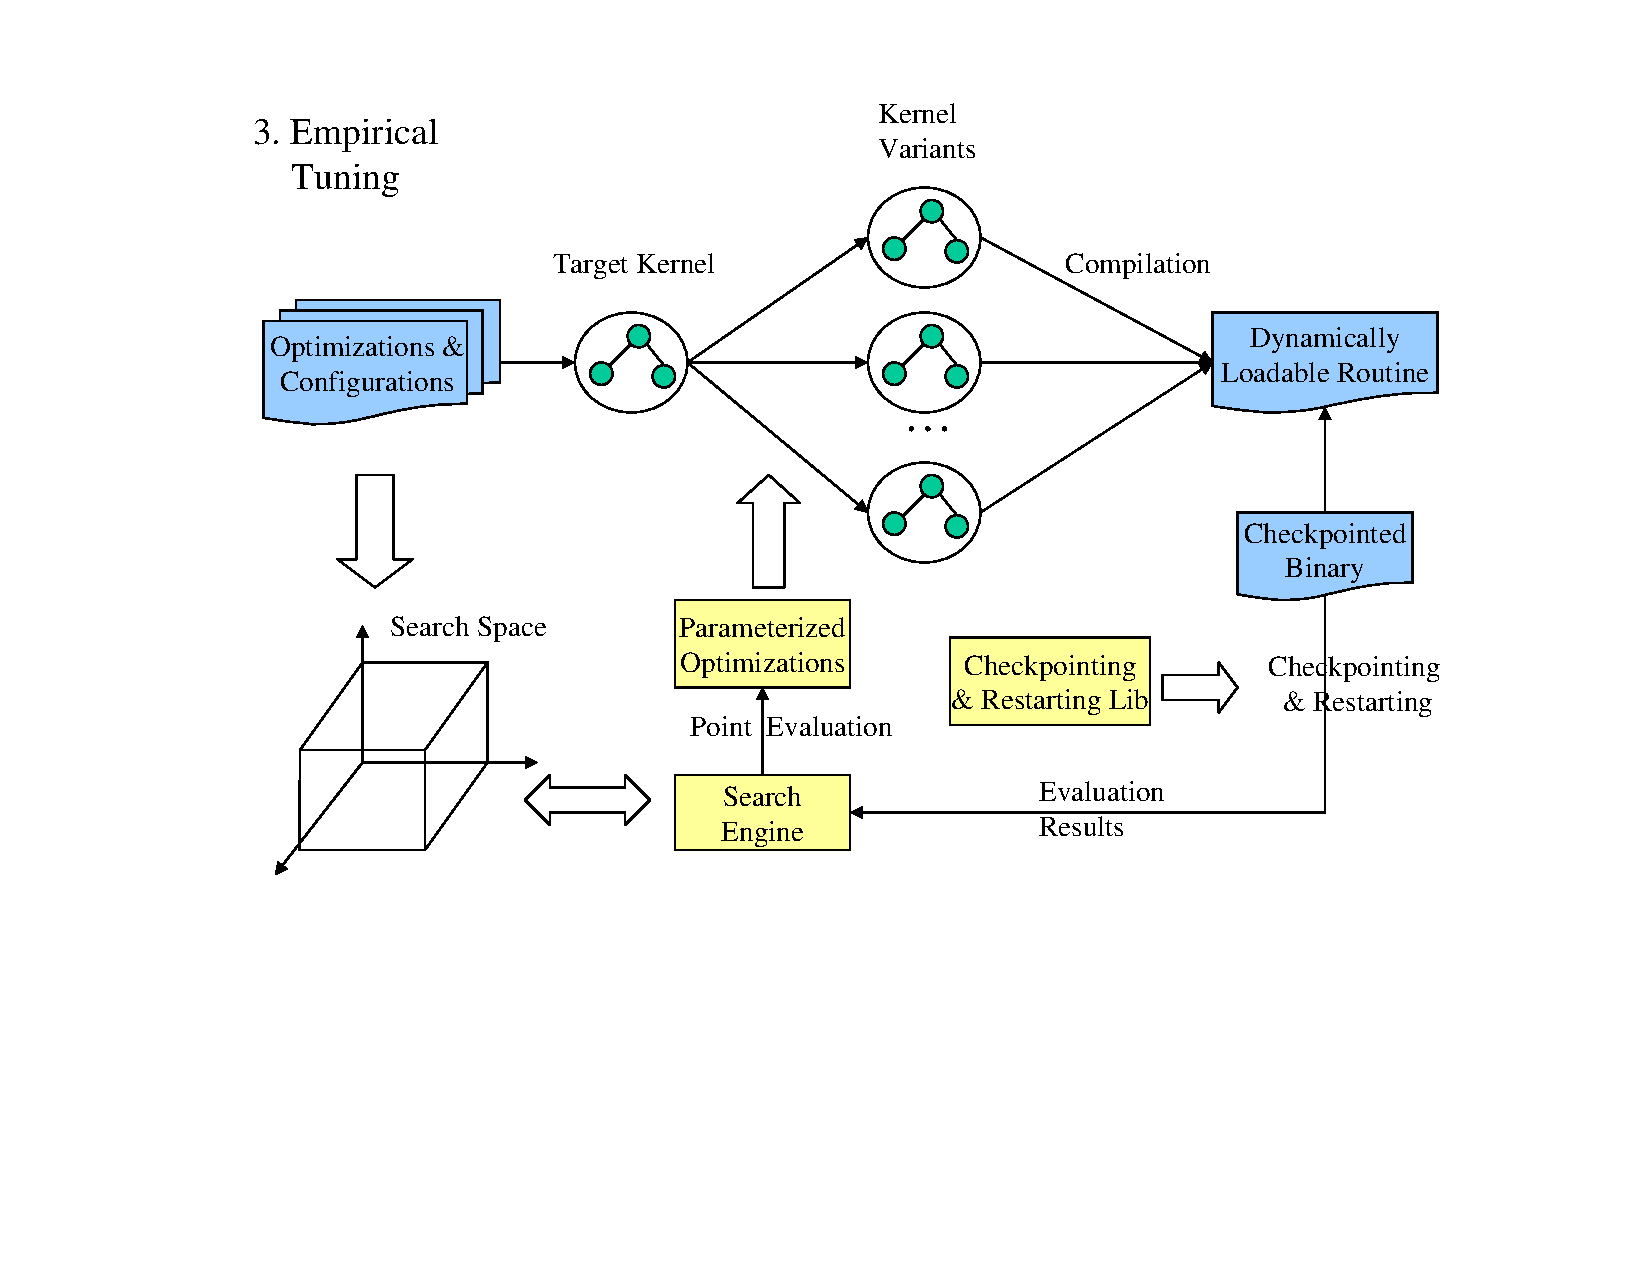
\includegraphics[width=1.2\textwidth]{phase3.pdf}
       \caption{Phase 3 of the autotuning system}
       \label{fig:phase3}
\end{figure}

%--------------------------------------------------
\subsection{Parameterized Transformation Tools}
Several choices exist to generate kernel variants, they include
POET~\cite{YiPOET2007},
CHiLL~\cite{ChenCHiLL2008}, and the ROSE loop translators. We take POET as an example here. 

POET (Parameterized Optimizations for Empirical
Tuning) developed by Dr.~Qing~Yi under contract with University of
Texas at San Antonio (UTSA), is an efficient language and tool to express hundreds or
thousands of complex code transformations and their configurations using a small set
of parameters.  It is especially relevant to the evaluation of large-scale search spaces
as part of empirical tuning and is orthogonal to any specific search strategy.

Using command line options and a configuration file, users can direct POET to apply a set
of specified transformations with desired configurations on selected code portions. 
Also, the target kernel has to be instrumented to aid POET in the process. 
Detailed POET user instructions can be found at its official website~\cite{poetWeb}.
For example, the SMG2000 kernel has the following format to support
POET:
\begin{figure}[!ht]
\centering
\lstset{language=C, basicstyle=\scriptsize}
\begin{lstlisting}
void
OUT__1__6755__ (void **__out_argv)
{
  int Ai =  *((int *)(__out_argv[20]));
  int xi =  *((int *)(__out_argv[19]));
  int ri =  *((int *)(__out_argv[18]));
  double *Ap =  *((double **)(__out_argv[17]));
  double *xp =  *((double **)(__out_argv[16]));
  double *rp =  *((double **)(__out_argv[15]));
  int loopi =  *((int *)(__out_argv[14]));
  int loopj =  *((int *)(__out_argv[13]));
  int loopk =  *((int *)(__out_argv[12]));
  int hypre__sx1 =  *((int *)(__out_argv[11]));
  int hypre__sy1 =  *((int *)(__out_argv[10]));
  int hypre__sz1 =  *((int *)(__out_argv[9]));
  int hypre__sx2 =  *((int *)(__out_argv[8]));
  int hypre__sy2 =  *((int *)(__out_argv[7]));
  int hypre__sz2 =  *((int *)(__out_argv[6]));
  int hypre__sx3 =  *((int *)(__out_argv[5]));
  int hypre__sy3 =  *((int *)(__out_argv[4]));
  int hypre__sz3 =  *((int *)(__out_argv[3]));
  int hypre__nx =  *((int *)(__out_argv[2]));
  int hypre__ny =  *((int *)(__out_argv[1]));
  int hypre__nz =  *((int *)(__out_argv[0]));
  for (loopk = 0; loopk < hypre__nz; loopk+=1) 
  {
    for (loopj = 0; loopj < hypre__ny; loopj+=1) 
    {
      for (loopi = 0; loopi < hypre__nx; loopi+=1)  //@BEGIN(nestI)
      {
        {
          rp[ri] -= ((Ap[Ai]) * (xp[xi]));
        }
        Ai += hypre__sx1;
        xi += hypre__sx2;
        ri += hypre__sx3;
      }
      Ai += (hypre__sy1 - (hypre__nx * hypre__sx1));
      xi += (hypre__sy2 - (hypre__nx * hypre__sx2));
      ri += (hypre__sy3 - (hypre__nx * hypre__sx3));
    }                                             //@END(nestI:Nest)
    Ai += (hypre__sz1 - (hypre__ny * hypre__sy1));
    xi += (hypre__sz2 - (hypre__ny * hypre__sy2));
    ri += (hypre__sz3 - (hypre__ny * hypre__sy3));
  }
 // some code omitted here...
}
\end{lstlisting}
  \caption{the SMG 2000 kernel}
    \label{Fig:smg2000kernel}
\end{figure}
%  for (loopk = 0; loopk < *hypre__nz; loopk+=1)
%    {
%      for (loopj = 0; loopj < *hypre__ny; loopj+=1)
%        {
%          for (loopi = 0; loopi < *hypre__nx; loopi+=1) //@BEGIN(nestI)
%            {
%              {
%                (*rp)[*ri] -= (((*Ap)[*Ai]) * ((*xp)[*xi]));
%              }
%              *Ai += *hypre__sx1;
%              *xi += *hypre__sx2;
%              *ri += *hypre__sx3;
%            }                                               //@END(nestI:Nest)
%          *Ai += (*hypre__sy1 - (*hypre__nx * *hypre__sx1));
%          *xi += (*hypre__sy2 - (*hypre__nx * *hypre__sx2));
%          *ri += (*hypre__sy3 - (*hypre__nx * *hypre__sx3));
%        }
%      *Ai += (*hypre__sz1 - (*hypre__ny * *hypre__sy1));
%      *xi += (*hypre__sz2 - (*hypre__ny * *hypre__sy2));
%      *ri += (*hypre__sz3 - (*hypre__ny * *hypre__sy3));
%    }
 
\fixme{TODO:the input is manually changed from the kernel generated by
the autoTuning translator. POET expects normalized loops
with special tags, integer loop control variables and $++$ operator is not allowed. 
We will discuss with Qing to either drop these restrictions or use ROSE to normalize
the loops automatically.}

The POET configuration file (my.pt) we use to optimize SMG2000's kernel is shown
below. In this file, loop unrolling is specified to be performed on the target
within a source file named out\_1\_6755\_\_.org.c. 
The result will be saved inside a file named out\_1\_6755\_\_c.
\lstset{basicstyle=\scriptsize}
\lstinputlisting{my.pt.fold}

A default transformation parameter, unrolling factor, is also given in the
file. But this parameter is usually superseded by a command line
parameter, the following command line specifies unrolling 5 times.
%The extracted kernel will be compiled as a dynamically loadable routine to
%be used by the target application. 
{\mySmallFontSize
\begin{verbatim}
/home/liao/download/qing/POET/src/pcg -punrollI=5 \
-L/home/liao/download/qing/POET/lib my.pt 
\end{verbatim}
}

\fixme{TODO The generation of .pt files it not yet automated currently.}

%--------------------------------------------------
\subsection{Search Engines}
Currently, we adopt the GCO (Generic Code Optimization) search engine~\cite{Youeffective2005} from University of Tennessee
at Knoxville as the external search engine used in our system.  
It has been connected with
a specific version of POET (not yet fully updated to the latest POET release
unfortunately) to explore code transformations using several popular search policies,
such as random search, exhaustive search, simulated anneal search, genetic algorithm,
and so on.

The search engine interacts with the parameterized optimization tool (POET)
via a bash script, usually named as eval\_xxx where xxx indicates the
target application.
This script is manually generated currently and does the following tasks:
\begin{enumerate}
   \item specifies the search space's dimension number and lower, upper bound
         for each dimension,
   \item specifies the number of executions for each evaluation. This will
         help exclude some executions disturbed by system noises, 
   \item validation of the number of command line options for this script, the
         number should match the number of dimensions of the search space so each
         value corresponding one dimension. All the options together mean a valid
         search point within the search space.
   \item converts the search point into transformation parameters
         understandable by POET. Some transformation choices are obtained by
         interpreting integer values in a custom way, such as the order of loop interchanging. 
   \item generates a kernel variant by invoking POET with right parameters to conduct the
         corresponding transformations on the target kernel,
   \item compiles the generated kernel variant into a dynamically loadable
         shared library file (a .so file),
   \item restarts the checkpointed binary to evaluate the kernel variant. This step is
         repeated multiple times as configured and the shortest execution time is reported as
         the evaluation result for this particular transformation setting (a point).
\end{enumerate}

A full example script for SMG2000 is given below.
\lstset{basicstyle=\scriptsize}
\lstinputlisting{eval_smg.fold}
\lstset{basicstyle=\small}

As we can see, the evaluation of a kernel variant needs the cooperation of
three parties.
\begin{enumerate}
   \item the transformed target application providing a performance
         measurement (timing) for the call to the variant, 
   \item the \lstinline{eval_smg} script choosing the best execution after
         several times of execution using the same kernel variant,
   \item the search engine retrieving the information returned from
         \lstinline{eval_smg} as the evaluation result of a variant and proceeding
         the search accordingly.
\end{enumerate}

%---------------------------------------------------------------
\subsection{An Example Search}
   We use the random search policy of the UTK search engine to demonstrate a
sample search process. The search engine chooses the maximum evaluation value as the best
result by default. So a reciprocal of a timing result is indicated by an environment
variable \lstinline{GCO_SEARCH_MODE} to be the evaluation result.  The UTK search engine
also accepts a upper time limit for a search session.  We use 1 minute in this example by
adding 1 as the last parameter. 
%following \lstinline{eval_smg}.

{\mySmallFontSize
\begin{verbatim}
[liao@localhost smg2000]$ export GCO_SEARCH_MODE=reciprocal
[liao@localhost smg2000]$ ../search/random_search ./eval_smg 1
Checkpointing: restarting here ..
Case: ./eval_smg 12  --
Got the evaluation result: 50.7846
Checkpointing: restarting here ..
Case: ./eval_smg 13  --
Got the evaluation result: 49.65
Checkpointing: restarting here ..
Case: ./eval_smg 11  --
Got the evaluation result: 50.9502
Checkpointing: restarting here ..
Case: ./eval_smg 31  --
Got the evaluation result: 49.8107
Checkpointing: restarting here ..
Case: ./eval_smg 15  --
Got the evaluation result: 49.8703
Checkpointing: restarting here ..
Case: ./eval_smg 14  --
Got the evaluation result: 49.645
Checkpointing: restarting here ..
Case: ./eval_smg 25  --
Got the evaluation result: 50.0551
Checkpointing: restarting here ..
Case: ./eval_smg 18  --
Got the evaluation result: 49.7018
skipping already visited point 31 , value = 49.810719
Checkpointing: restarting here ..
Case: ./eval_smg 32  --
Got the evaluation result: 49.5221
Checkpointing: restarting here ..
Case: ./eval_smg 22  --
Got the evaluation result: 49.6475
Checkpointing: restarting here ..
Case: ./eval_smg 6  --
Got the evaluation result: 51.261
Checkpointing: restarting here ..
Case: ./eval_smg 30  --
Got the evaluation result: 50.0475
skipping already visited point 18 , value = 49.701789
skipping already visited point 14 , value = 49.645038
Checkpointing: restarting here ..
Case: ./eval_smg 4  --
Got the evaluation result: 51.435
Time limit reached...
---------------------------------------------------
Random Search Best Result:  Value=49.522112, Point=32
Total Number of evaluations: 13

\end{verbatim}
}

In the sample search above, a one-dimension search space (loop unrolling
factor) was examined.  
Within the one-minute time limit, points were randomly chosen by the
search engine and three of them were redundant. 
Apparently, the UTK search engine was able to skip redundant evaluations.
In the end, a point (32) had the best value (reciprocal of timing) which
means for the target smg2000 kernel, unrolling 32 times generated the best
performance.

Similarly, other search policies can be used by replacing
\lstinline{random_search} with
\lstinline{exhaustive_search}, \lstinline{anneal_search},
\lstinline{ga_search}, \lstinline{simplex_search}, etc. 

\section{Working with Active Harmony}
We describe how our end-to-end empirical tuning framework can be adapted to work with another search engine, namely the Active Harmony system~\cite{TapusActive2002,ChungCase2006}. 
The work is done with generous help from Ananta Tiwari at University of
Maryland.

Active Harmony allows online, runtime tuning of application parameters which are critical to the application performance. 
Domain-specific knowledge is usually needed to identify those application parameters.
An active harmony server will be running to manage the values of different application parameters and to conduct the search.
Applications have to be modified to communicate with the server in order to send performance feedback for one specific set of parameter values (current point) and get the next set of parameter values (next point).
Currently, it supports a search strategy based on the Nelder-Mead simplex method~\cite{NelderSimplex1965}.

For SMG2000, we generate a set of unrolled versions (OUT\_\_1\_\_6755\_\_X()) for the target kernel and treat the function suffix X as the tunable parameter. 
As a result, the .so file contains all unrolled versions.
\fixme{This is not an ideal way to tune the application, we will explore better alternatives.}

%TODO add the tcl configuration file here
A configuration file is needed for Active Harmony to know the parameters to
be tuned and their corresponding ranges. 
The following file is used to specify a tunable parameter named unroll with a range from 1 to 32.
obsGoodness (observed Goodness - or performance) and predGoodness (predicted goodness) are related to a GUI window showing during the execution. 
They do not impact the performance tuning and the workings of the search algorithm. 
{\mySmallFontSize
\begin{verbatim}
harmonyApp smg2000Unroll {
   { harmonyBundle unroll {
       int {1 32 1}
   }
   }
    { obsGoodness 1 5000}
    { predGoodness 1 5000}
}
\end{verbatim}
}

We don't use BLCR since an online tuning method is used for Active Harmony. 
The code transformation to work with Active Harmony is shown below.
The basic idea is to call a set of Harmony interface functions to startup communication with the server (\lstinline{harmony_startup()}),
send a configuration file (\lstinline{harmony_application_setup_file()}), define a parameter to be tuned (\lstinline{harmony_add_variable(})),  report performance feedback (\lstinline{harmony_peformance_update()}), 
and finally request the next set of values of the tunable parameters (\lstinline{harmony_request_all()}).
\lstset{language={C},basicstyle=\scriptsize}
\lstinputlisting{smg2000_harmony.c}
\lstset{language={C},basicstyle=\small}

Figure~\ref{fig:activeHarmony2} shows a screen shot of using Active Harmony to tuning the SMG2000 benchmark. 
The top panel gives a graphical representation of the search space (one dimension named unroll) and the tuning timeline with evaluation values (x-axis is time, y-axis is evaluation values). 
The left-bottom shell window is the client application being tuned. 
The right-bottom shell windows shows the activities of the server.
\begin{figure}[tbp]
        \centering
                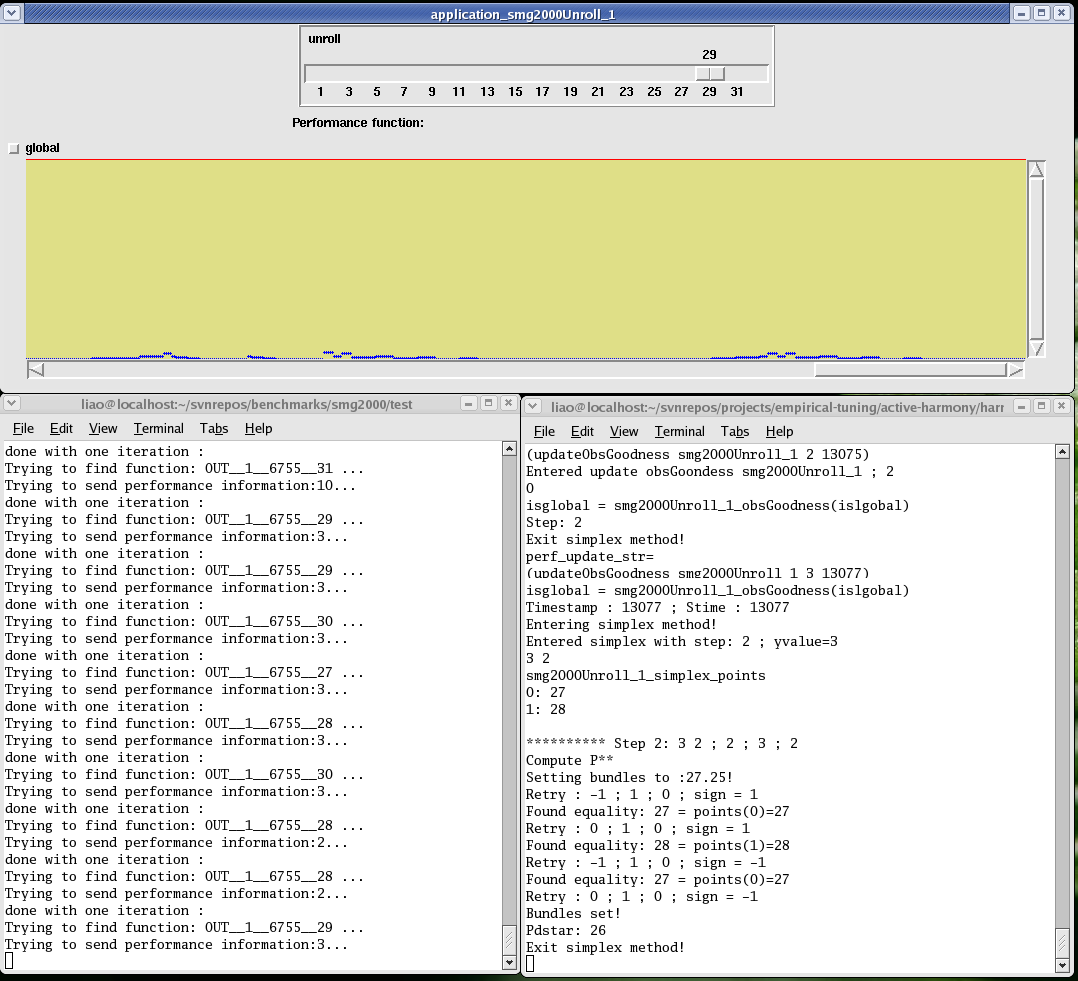
\includegraphics[width=0.8\textwidth]{activeHarmony2.png}
        \caption{Searching using Active Harmony}
        \label{fig:activeHarmony2}
\end{figure}

We have found that online/runtime search engines like the Active Harmony can be extremely expensive if the tuned kernel are invoked thousands of times. 
For SMG2000, it took hours to finish the tuning using a 120x120x120 input data set.
The major reason is that for each call of the kernel, a bidirectional communication between the client application and the server has to be finished. 
Another reason is that the current tuning process is embedded into the thousands of calls of the kernel so that points are always evaluated even when some of them have already been evaluated before. 



\clearpage
\section{User-Directed Autotuning}
While fully automated autotuning can be feasible in some cases, many
applications need users' expertise to obtain significant performance improvements. 
We revisit the SMG2000 benchmark in this section to see how one can use our autotuning system to have a user-directed empirical tuning process.
%-------------------------------------
\subsection{Manual Code Triage}
The SMG2000 kernel (shown in Fig.~\ref{Fig:smg2000kernel}) that is automatically identified by our simple code triage may not be the best tuning target. 
It is actually only a portion of a bigger computation kernel that is very
hard to be automatically identified. 
Also, the bigger kernel has a very complex form which impedes most
compilers or tools for further analyses and transformations. 
With the help from Rich Vuduc, who is a former postdoc with us, we manually transform the code (via code specification) to obtain a representative kernel which captures the core computation algorithm of the benchmark. 
We then put the outlining pragma (\lstinline{#pragma rose_outline}) before
the new kernel and invoked the ROSE outliner to separate it out into a new
source file, as shown below.

\lstset{language=C, basicstyle=\scriptsize}
\begin{lstlisting}
#include "autotuning_lib.h"
static double time1, time2;
void OUT__1__6119__(void **__out_argv);
typedef int hypre_MPI_Comm;
typedef int hypre_MPI_Datatype;
typedef int hypre_Index[3];

typedef struct hypre_Box_struct
{
   hypre_Index imin;
   hypre_Index imax;
} hypre_Box;

typedef struct hypre_BoxArray_struct
{
   hypre_Box *boxes;
   int size;
   int alloc_size;
} hypre_BoxArray;

typedef struct hypre_RankLink_struct
{
   int rank;
   struct hypre_RankLink_struct *next;
} hypre_RankLink;

typedef hypre_RankLink *hypre_RankLinkArray[3][3][3];

typedef struct hypre_BoxNeighbors_struct
{
   hypre_BoxArray *boxes;
   int *procs;
   int *ids;
   int first_local;
   int num_local;
   int num_periodic;
   hypre_RankLinkArray *rank_links;
} hypre_BoxNeighbors;

typedef struct hypre_StructGrid_struct
{
   hypre_MPI_Comm comm;
   int dim;
   hypre_BoxArray *boxes;
   int *ids;
   hypre_BoxNeighbors *neighbors;
   int max_distance;
   hypre_Box *bounding_box;
   int local_size;
   int global_size;
   hypre_Index periodic;
   int ref_count;
} hypre_StructGrid;

typedef struct hypre_StructStencil_struct
{
   hypre_Index *shape;
   int size;
   int max_offset;
   int dim;
   int ref_count;
} hypre_StructStencil;

typedef struct hypre_CommTypeEntry_struct
{
   hypre_Index imin;
   hypre_Index imax;
   int offset;
   int dim;
   int length_array[4];
   int stride_array[4];
} hypre_CommTypeEntry;

typedef struct hypre_CommType_struct
{
   hypre_CommTypeEntry **comm_entries;
   int num_entries;
} hypre_CommType;

typedef struct hypre_CommPkg_struct
{
   int num_values;
   hypre_MPI_Comm comm;
   int num_sends;
   int num_recvs;
   int *send_procs;
   int *recv_procs;
   hypre_CommType **send_types;
   hypre_CommType **recv_types;
   hypre_MPI_Datatype *send_mpi_types;
   hypre_MPI_Datatype *recv_mpi_types;
   hypre_CommType *copy_from_type;
   hypre_CommType *copy_to_type;
} hypre_CommPkg;

typedef struct hypre_StructMatrix_struct
{
  hypre_MPI_Comm comm;
  hypre_StructGrid *grid;
  hypre_StructStencil *user_stencil;
  hypre_StructStencil *stencil;
  int num_values;
  hypre_BoxArray *data_space;
  double *data;
  int data_alloced;
  int data_size;
  int **data_indices;
  int symmetric;
  int *symm_elements;
  int num_ghost[6];
  int global_size;
  hypre_CommPkg *comm_pkg;
  int ref_count;
} hypre_StructMatrix;

void OUT__1__6119__(void **__out_argv)
{
  static int counter =0 ;
  hypre_StructMatrix *A =  *((hypre_StructMatrix **)(__out_argv[20]));
  int ri =  *((int *)(__out_argv[19]));
  double *rp =  *((double **)(__out_argv[18]));
  int stencil_size =  *((int *)(__out_argv[17]));
  int i =  *((int *)(__out_argv[16]));
  int (*dxp_s)[15UL] = (int (*)[15UL])(__out_argv[15]);
  int hypre__sy1 =  *((int *)(__out_argv[14]));
  int hypre__sz1 =  *((int *)(__out_argv[13]));
  int hypre__sy2 =  *((int *)(__out_argv[12]));
  int hypre__sz2 =  *((int *)(__out_argv[11]));
  int hypre__sy3 =  *((int *)(__out_argv[10]));
  int hypre__sz3 =  *((int *)(__out_argv[9]));
  int hypre__mx =  *((int *)(__out_argv[8]));
  int hypre__my =  *((int *)(__out_argv[7]));
  int hypre__mz =  *((int *)(__out_argv[6]));
  int si =  *((int *)(__out_argv[5]));
  int ii =  *((int *)(__out_argv[4]));
  int jj =  *((int *)(__out_argv[3]));
  int kk =  *((int *)(__out_argv[2]));
  const double *Ap_0 =  *((const double **)(__out_argv[1]));
  const double *xp_0 =  *((const double **)(__out_argv[0]));

  at_begin_timing(); // begin timing

  for (si = 0; si < stencil_size; si++)
    for (kk = 0; kk < hypre__mz; kk++)
      for (jj = 0; jj < hypre__my; jj++)
        for (ii = 0; ii < hypre__mx; ii++)
          rp[(ri + ii) + (jj * hypre__sy3) + (kk * hypre__sz3)] -= 
             Ap_0[ii + (jj * hypre__sy1) + (kk * hypre__sz1) +  A -> data_indices[i][si]] *
             xp_0[ii + (jj * hypre__sy2) + (kk * hypre__sz2) + ( *dxp_s)[si]];
  at_end_timing(); //end timing

   *((int *)(__out_argv[2])) = kk;
   *((int *)(__out_argv[3])) = jj;
   *((int *)(__out_argv[4])) = ii;
   *((int *)(__out_argv[5])) = si;
   *((double **)(__out_argv[18])) = rp;
   *((hypre_StructMatrix **)(__out_argv[20])) = A;
}

\end{lstlisting}

As we can see, the new kernel directly and indirectly depends on some user defined types. 
The ROSE outliner was able to recursively find and copy them into the new
file in a right order.
%The header (autotuning\_lib.h) provides prototypes of timing and checkpointing/restarting 
%-------------------------------------------------------------
\subsection{Parameterized ROSE Loop Translators}
ROSE provides several standalone executable programs
(loopUnrolling, loopInterchange, and loopTiling under ROSE\_INSTALL/bin) for loop
transformations.
So autotuning users can use them via command
lines with abstract handles to create desired kernel variants.
Detailed information about the parameterized loop translators can be found
in Chapter 50 of the \htmladdnormallink{ROSE
Tutorial}{http://www.rosecompiler.org/ROSE_Tutorial/ROSE-Tutorial.pdf}.


These translators use ROSE's internal loop translation interfaces (declared within the SageInterface namespace). They are:

\begin{itemize}
\item \textit{bool loopUnrolling (SgForStatement *loop, size\_t
unrolling\_factor)}:
This function needs two parameters: one for the loop to be
unrolled and the other for the unrolling factor.
\item \textit{bool  loopInterchange (SgForStatement *loop, size\_t depth,
size\_t lexicoOrder)}:
The loop interchange function has three parameters, the first one to
specify a loop which starts a perfectly-nested loop and is to be
interchanged, the 2nd for the depth of the loop nest to be interchanged, and finally the
lexicographical order for the permutation.
\item \textit{bool  loopTiling (SgForStatement *loopNest, size\_t
targetLevel, size\_t tileSize)}:
The loop tiling interface needs to know the loop nest to be tiled, which
loop level to tile, and the tile size for the level.
\end{itemize}
For efficiency concerns, these functions only perform the specified
translations without doing any legitimacy check.
It is up to the users to
make sure the transformations won't generate wrong code.
%We will soon provide interfaces to do the eligibility check for each transformation.

Example command lines using the programs are given below:

{\scriptsize
\begin{verbatim}
# unroll a for statement 5 times. The loop is a statement at line 6 within an input file.

loopUnrolling -c inputloopUnrolling.C \
-rose:loopunroll:abstract_handle "Statement<position,6>" -rose:loopunroll:factor 5

# interchange a loop nest starting from the first loop within the input file,
# interchange depth is 4 and
# the lexicographical order is 1 (swap the innermost two levels)

loopInterchange -c inputloopInterchange.C -rose:loopInterchange:abstract_handle \
"ForStatement<numbering,1>" -rose:loopInterchange:depth 4 \
-rose:loopInterchange:order 1

# tile the loop with a depth of 3 within the first loop of the input file
# tile size is 5

loopTiling -c inputloopTiling.C -rose:loopTiling:abstract_handle \
"ForStatement<numbering,1>" -rose:loopTiling:depth 3 -rose:loopTiling:tilesize 5

\end{verbatim}
}

%-------------------------------------------------------------
\subsection{Connecting to the Search Engine}
We applied several standard loop optimizations to the new kernel.
They are, in the actual order applied,
loop tiling on i, j and k levels (each level has a same tiling size from 0
to 55 and a stride of 5),
loop interchange of i, j, k and si levels (with a lexicographical permutation order ranging from 0 to 4! -1),
and finally loop unrolling on the innermost loop only.
For all optimizations, a parameter
value of 0 means no such optimization is applied.
So the total search space has 14400 ($12*4!*50$) points.

The bash script used by the GCO search engine to conduct point evaluation is given blow. 
Note that a transformation command needs to consider previous transformations' side effects on the kernel. 
We also extended GCO to accept strides (using \textit{\#ST} in the script) for dimensions of search space.  
{\scriptsize
\begin{verbatim}  
$ cat eval_smg_combined
#!/bin/bash
#DIM    3
#LB     0 0 0
#UB     55 23 49
#ST     5 1 1

# number of executions to find the best result for this variant
ITER=3

# command line validation
# should have x parameters when calling this script
# x= number of dimensions for each point
if [ "$3" = "" ]; then
  echo "Fatal error: not enough  parameters are provided for all search dimensions"
  exit
fi

# convert points to transformation parameters
# Not necessary in this example

# target application path
APP_PATH=/home/liao6/svnrepos/benchmarks/smg2000
KERNEL_VARIANT_FILE=OUT__1__6119__.c
# remove previous variant of the kernel and result
/bin/rm -f $APP_PATH/struct_ls/$KERNEL_VARIANT_FILE /tmp/peri.result $APP_PATH/*.so *.so

# ------------ tiling i, j, k ----------------------
# first tiling is always needed.
loopTiling -c $APP_PATH/struct_ls/OUT__1__6119__perfectNest.c  -rose:loopTiling:abstract_handle "ForStatement<numbering,1>"\
 -rose:loopTiling:depth 4 -rose:loopTiling:tilesize $1 -rose:output $KERNEL_VARIANT_FILE

if [ $1 -ne 0 ]; then
loopTiling -c $KERNEL_VARIANT_FILE -rose:loopTiling:abstract_handle "ForStatement<numbering,1>" -rose:loopTiling:depth 4 \
-rose:loopTiling:tilesize $1 -rose:output $KERNEL_VARIANT_FILE loopTiling -c $KERNEL_VARIANT_FILE \
-rose:loopTiling:abstract_handle "ForStatement<numbering,1>" -rose:loopTiling:depth 4 -rose:loopTiling:tilesize $1 \
-rose:output $KERNEL_VARIANT_FILE

fi
# -------------- interchange si, k, j, i--------------
if [ $1 -ne 0 ]; then
loopInterchange -c $KERNEL_VARIANT_FILE -rose:output $KERNEL_VARIANT_FILE \
-rose:loopInterchange:abstract_handle 'ForStatement<numbering,4>' \
 -rose:loopInterchange:depth 4 -rose:loopInterchange:order $2
else
# No tiling happens, start from 1
loopInterchange -c $KERNEL_VARIANT_FILE -rose:output $KERNEL_VARIANT_FILE \
-rose:loopInterchange:abstract_handle 'ForStatement<numbering,4>' \
-rose:loopInterchange:depth 1 -rose:loopInterchange:order $2
fi

# ------------ unrolling innermost only -------------------
# generate a variant of the kernel using the transformation parameters
# unrolling the innermost level, must redirect to avoid mess up search engine
if [ $1 -ne 0 ]; then
loopUnrolling -c $KERNEL_VARIANT_FILE  -rose:loopunroll:abstract_handle "ForStatement<numbering,7>" \
-rose:loopunroll:factor $3 -rose:output $KERNEL_VARIANT_FILE > /dev/null 2>&1
else
loopUnrolling -c $KERNEL_VARIANT_FILE  -rose:loopunroll:abstract_handle "ForStatement<numbering,4>" \
-rose:loopunroll:factor $3 -rose:output $KERNEL_VARIANT_FILE > /dev/null 2>&1
fi

# build a .so for the kernel variant
# To redirect stdout to NULL is required
# since the search engine looks for stdout for the evaluation result
make -f makefile-lib  filename=OUT__1__6119__ > /dev/null 2>&1
cp OUT__1__6119__.so $APP_PATH/struct_ls/.

# generate a program to execute and timing the kernel
# Handled by ROSE

best_time="999999999.0"

# run the program multiple times
for (( i="1" ; i <= "$ITER" ; i = i + "1" ))
do

  # The tuned kernel will write timing information into /tmp/peri.result
   $APP_PATH/test/smg2000 -n 120 120 120 -d 3 > /dev/null 2>&1
  if [ $? -ne 0 ]; then
    echo "Error: program finishes abnormally!"
    exit 1
  else
    test -f /tmp/peri.result
    if [ $? -ne 0 ]; then
       echo "Error: The temp file storing timing information does not exist!"
       exit 1
    fi
    time=`tail -1 /tmp/peri.result | cut -f 1`
# select the smaller one
    best_time=`echo ${time} ${best_time} | awk '{print ($1 < $2) ? $1 : $2}'`
  fi
  # remove the temp file, the best time is kept by the script already
  /bin/rm -f  /tmp/peri.result
done

# report the evaluation result to the search engine
echo $best_time

\end{verbatim}
} % end scriptsize
%-------------------------------------------------------------
\subsection{Results}
%With the help from the checkpointing/restarting library and 
The new SMG2000 kernel is invoked thousands of times during a typical execution.
So instead of using checkpointing/restarting, we used a counter to reduce
the point evaluation time. The counter was set to be 1600, which means the
execution is terminated once the kernel is be called 1600 times.
By doing this, an exhaustive search using GCO
became feasible within 40 hours for an input data size of $120*120*120$.

The best performance was achieved at point (0,8,0), which means loop
interchange using the lexicographical number 8 (corresponding to an order of $[k,j,si,i]$) improved the
performance while tiling and unrolling did not help at all.
The best searched point achieved a 1.43x speedup for the kernel (1.18 for the whole
benchmark) when compared to the execution time using Intel C/C++ compiler v. 9.1.045 with option \textit{-O2}
on the Dell T5400 workstation.



\section{Summary}

   The work presented is ongoing work, and focused on the whole program empirical tuning
and the automation of all the required steps to make that work for realistic HPC applications
in C, C++, and Fortran.  
The work to has a few steps that are likely not so easy to fully
automate, namely the manipulation of the Makefiles and bash scripts that are required to support the empirical
tuning, but it is likely this can be simplified in the future.

The work presented is also immediately focused on providing an infrastructure for 
the empirical tuning and less on the empirical tuning of any specific applications.
SMG2000 was selected somewhat at random, since it is moderately large and 
we have demonstrated for many years that we can compile it easily with ROSE.


% just put it here temporarily
\clearpage
\section{Appendix}
This section gives quick instructions for installing some needed software packages to establish the end-to-end autotuning system. 
Please consult individual software releases for detailed installation guidance. 

\subsection{Patching Linux Kernels with perfctr}
This is required before you can install PAPI on Linux/x86 and Linux/x86\_64 platforms. 
Take PAPI 3.6.2 as an example, the steps to patch your kernel are:
\begin{itemize}
\item Find the latest perfctr patch which matches your Linux distribution from \textit{papi-3.6.2/src/perfctr-2.6.x/patches}. 
For Red Hat Enterprise Linux 5 (or CentOS 5), the latest kernel patch is \textit{patch-kernel-2.6.18-92.el5-redhat}.
\item Get the Linux kernel source rpm package which matches the perfctr kernel patch found in
the previous step. 
You can find kernel source rpm packages from one of the many mirror sites. For example, 
\textit{wget http://altruistic.lbl.gov/mirrors/centos/5.2/updates/SRPMS/kernel-2.6.18-92.1.22.el5.src.rpm}
\item Install the kernel source rpm package. With a root privilege, simply type: 
\begin{verbatim}
rpm -ivh kernel*.src.rpm
\end{verbatim}
The command will generate a set of patch files under
\textit{/usr/src/redhat/SOURCES}.
\item Generate the kernel source tree from the patch files. 
This step may require the \textit{rpm-build} and \textit{redhat-rpm-config} packages to be installed first. 
\begin{verbatim}
yum install rpm-build redhat-rpm-config      # with the root privilege 
cd /usr/src/redhat/SPECS
rpmbuild -bp --target=i686 kernel-2.6.spec   # for x86 platforms    
rpmbuild -bp --target=x86_64 kernel-2.6.spec #for x86_64 platforms
\end{verbatim}

\item Copy the kernel source files and create a soft link. Type 
\begin{verbatim}
cp -a /usr/src/redhat/BUILD/kernel-2.6.18/linux-2.6.18.i686 /usr/src
ln -s /usr/src/linux-2.6.18.i686 /usr/src/linux
\end{verbatim}

\item Now you can patch the kernel source files to support perfctr. Type 
\begin{verbatim}
cd /usr/src/linux
/path/to/papi-3.6.2/src/perfctr-2.6.x/update-kernel \
     --patch=2.6.18-92.el5-redhat
\end{verbatim}

\item Configure your kernel to support hardware counters.
\begin{verbatim}
cd /usr/src/linux 
make clean
make mrproper 
yum install ncurses-devel 
make menuconfig
\end{verbatim}
Enable all items for \textit{performance-monitoring counters support} under the menu item of \textit{processor type and features}.
\item Build and install your patched kernel. 
\begin{verbatim}
make -j4 && make modules -j4 && make modules_install && make install
\end{verbatim}
\item Configure perfctr as a device that is automatically loaded each time you boot up your machine.
\begin{verbatim}
cd /home/liao6/download/papi-3.6.2/src/perfctr-2.6.x
cp etc/perfctr.rules /etc/udev/rules.d/99-perfctr.rules
cp etc/perfctr.rc /etc/rc.d/init.d/perfctr
chmod 755 /etc/rc.d/init.d/perfctr
/sbin/chkconfig --add perfctr
\end{verbatim}
\end{itemize}
With the kernel patched, it is straightforward to install PAPI. 
\begin{verbatim}
cd /home/liao6/download/papi-3.6.2/src
./configure
make
make test
make install # with a root privilege
\end{verbatim}
%----------------------------------------------
\subsection{Installing BLCR}
BLCR (the Berkeley Lab Checkpoint/Restart library)'s installation guide can be found at
\url{http://upc-bugs.lbl.gov/blcr/doc/html/BLCR_Admin_Guide.html}.
We complement the guide with some Linux-specific information here.
It is recommended to use a separate build tree to compile the library.
\begin{verbatim}
mkdir buildblcr
cd buildblcr
# explicitly provide the Linux kernel source path 
../blcr-0.8.2/configure --with-linux=/usr/src/linux-2.6.18.i686
make
# using a root account
make install
make insmod check

# Doublecheck kernel module installation 
# You should find two module files: blcr_imports.ko blcr.ko 
ls /usr/local/lib/blcr/2.6.18-prep/ 
\end{verbatim}
To configure your system to load BLCR kernel modules at bootup:
\begin{verbatim}
# copy the sample service script to the right place
cp blcr-0.8.2/etc/blcr.rc /etc/init.d/.
# change the module path inside of it 
vi /etc/init.d/blcr.rc
  #module_dir=@MODULE_DIR@
  module_dir=/usr/local/lib/blcr/2.6.18-prep/
#run the blcr service each time you boot up your machine
chkconfig --level 2345 blcr.rc on

# manually start the service 
# error messages like "FATAL: Module blcr not found." can be ignored. 
/etc/init.d/blcr.rc restart
Unloading BLCR: FATAL: Module blcr not found.
FATAL: Module blcr_imports not found.
                                                           [  OK  ]
Loading BLCR: FATAL: Module blcr_imports not found.
FATAL: Module blcr not found.
                                                           [  OK  ]

\end{verbatim}



\bibliographystyle{plain}
\bibliography{minidb}
\listoffixmes
\end{document}

%
